\chapter{Test Cases and Results}
\label{sec:results}

In this chapter we present the test case scenarios simulated in this work as well as
the results of the various simulations performed. First, a description of the 
scenarios is given to detail the geometry and cross section configurations used. 
Next, a comparison of deterministic results for the test scenarios is given, with 
discussion and emphasis placed on the difference in the results between different 
types of quadrature sets. Then, we present results and analysis of the performance of
the quadrature sets' associated Monte Carlo variance reduction parameters in the
context of both CADIS and \fwc\ simulations. Finally, a summary of the results is
given to conclude the chapter.

\section{Test Case Scenarios}

\subsection{Steel Plate in Water}
\label{sec:steel_params}

The first test case we describe is an idealized geometry of a steel plate embedded in
water; it is modeled after the scenario presented in Reference 
\cite{wilsonslaybaugh}. 
A diagram of the problem geometry is shown in Figure \ref{steelxz} and a list
of material properties used in the problem is given in Table \ref{steel-mat}.
In Figure \ref{steelxz}, the orange region contains the source material, the black
region is composed of steel, the blue regions indicate water, and the white region is
composed of air.

\begin{figure}[!htb]
\centering
\includegraphics[width=0.4\textwidth]{img/steel-xz.png}
\caption{Steel plate in water geometry ($x-z$ slice through $y = 25$ cm) 
         \cite{wilsonslaybaugh}.}
\label{steelxz}
\end{figure}

The problem measurements are $53\times50\times140$ cm. The scenario is uniform in the 
$y$-direction and materials vary mainly in the $z$-direction. The source region 
extends from 0 to 15 cm, the steel shield extends between 15 and 30 cm, the water and 
steel plate extend from 30 to 130 cm, and the air extends from 130 to 140 cm. The 
steel plate is 3 cm wide and is centered at $x = 26.5$ cm. Vacuum boundary conditions 
were used at the problem boundaries.

A non-uniform Cartesian mesh was used for the spatial discretization in the 
deterministic calculations. In the $x$-direction, voxel width is 5 cm between $x = 0$
cm and $x = 25$ cm, 0.5 cm between $x = 25$ cm and $x = 28$ cm, and 5 cm between 
$x = 28$ cm and $x = 53$ cm. A uniform spacing of voxel width 1 cm was used in the 
$y$-direction. In the $z$-direction, the spatial cell width is 3 cm between $z = 0$ cm and
$z = 30$ cm and 2 cm between $z = 30$ cm and $z = 140$ cm.

\begin{table}[!htb]
\centering
\caption{Materials and compositions in the steel plate in water scenario.}
\label{steel-mat}
\begin{tabular}{l|cc}
\textbf{Material} & \multicolumn{2}{c}{\textbf{Isotopes (Atomic \%)}} \\ \hline
\multirow{5}{*}{Source}   & U-235   & (0.000247) \\
                          & U-238   & (0.009287) \\
                          & Zr-nat. & (0.004009) \\
                          & H-1     & (0.037394) \\
                          & O-16    & (0.034927) \\ \hline
\multirow{4}{*}{Air}      & N-14    & (0.784431) \\
                          & O-16    & (0.210748) \\
                          & Ar-nat. & (0.004671) \\
                          & C-nat.  & (0.000150) \\ \hline
\multirow{2}{*}{Carbon Steel} & C-nat.  & (0.022831) \\
                              & Fe-nat. & (0.977169) \\ \hline
\multirow{2}{*}{Water}        & H-1     & (2)        \\
                              & O-16    & (1)        \\
\end{tabular}
\end{table}

The composition of the neutron source block is a homogenization of water, zirconium,
and uranium and was calculated based on the geometry and composition of the Rowlands
UO$_2$ pin cell benchmark specification \cite{pincell}. The source is a U-235 fission 
spectrum that is uniformly distributed throughout the homogenized material. The
compositions of air, carbon steel, and water were taken from the Compendium of 
Material Composition Data for Radiation Transport Modeling \cite{pnnl}. For this scenario,
we are interested in the forward flux solutions at the end of the steel plate.

\FloatBarrier
\subsection{Dog-Legged Void Neutron (DLVN)}

The next problem modeled is the dog-legged void neutron (DLVN) experimental benchmark,
which was designed to measure neutron streaming in iron with air voids. The model used
in the following calculations was constructed from References 
\cite{sw-dlvn,j-dlvn,dlvn1991}. The two materials used in the problem are elemental 
iron and polyethylene. The polyethylene composition used was C$_2$H$_4$. This is 
listed as ``polyethylene, non-borated'' and is material 248 in Reference \cite{pnnl}. 

\begin{figure}[!htb]
\centering
\includegraphics[width=0.5\textwidth]{img/dlvn.png}
\caption{Centerline cutaway of DLVN setup \cite{sw-dlvn}.}
\label{dlvn}
\end{figure}

The problem measurements are $40\times54\times48$ inches. A uniform spatial mesh was 
imposed over the entire problem, with voxels measuring 1 inch per side. The neutron
source in this problem is a Cf-252 point source located at the center of the $x-$ and
$y-$directions and at $z = 9$ inches. For reasons noted in Section \ref{sec:ptsrc},
this point source was approximated as a small volumetric source in the tests in this 
work. We are interested in the forward flux solutions at the various detector locations
shown in Figure \ref{dlvn}.

The experimental configuration is symmetric about the $y-z$ plane at $x = 0$ and so is
usually simulated with a reflecting boundary at $x = 0$ and vacuum boundaries on all
other sides of the configuration. For the tests in this work, the use of reflecting
boundary conditions was not available (see Section \ref{sec:bc}), so the model used 
was constructed to represent the entire experimental geometry configuration. Vacuum
boundary conditions were applied to the outside of the entire problem.

\FloatBarrier
\subsection{Ispra Sodium Benchmark}

The Ispra sodium benchmark experiment was constructed as part of experiments to study
neutron deep penetration in homogeneous materials commonly used in advanced nuclear
reactors. It is included in the Shielding Integral Benchmark Archive and Database 
(SINBAD) data library \cite{sinbad}. We will give a brief overview of the material and
geometry configuration here and refer the reader to Reference \cite{sinbad} for a 
complete description of the experiment.

The neutron source consists of fission neutrons originating from an enriched U disc 
that was subjected to a neutron flux leaving the thermal column of a TRIGA MARK II 
reactor. An irradiation tunnel assembly composed of steel containers filled with Na 
was constructed in front of the neutron source converter. The total length of the 
irradiation tunnel was 400 cm. A diagram of the experimental geometry is shown in 
Figure \ref{eurac}; we are interested in the forward flux solutions in the detector
array located along the midline of the assembly.

\begin{figure}[!htb]
\centering
\includegraphics[width=\textwidth]{img/eurna-2v.png}
\caption{Cross sectional views of the sodium benchmark assembly.}
\label{eurac}
\end{figure}

In the simulation of this benchmark configuration, the boundaries are -300 cm and 500
cm in the $x-$direction and -400 and 400 cm in both the $y-$ and $z-$directions.
The spatial mesh in this problem is uniform in the $y-$ and $z-$directions with a 
voxel width of 5 cm per side in these dimensions. The $x-$direction mesh was 
created such that voxels are 10 cm wide between $x =$ -300 and -100 cm, 5 cm wide 
between $x =$ -100 and 400 cm, and 10 cm wide between $x =$ 400 and 500 cm. The problem
has vacuum boundary conditions.

\FloatBarrier
\subsection{Simplified Portal Monitor}

The final problem described here is a simplified portal monitor scenario. Portal
monitors are large detector panels used to screen cargo for illicit radioactive
materials. The problem models a cargo container holding a Ba-133 photon point source
and large blocks of homogenized iron and polyethylene. 
The geometry and material configuration used in this test is the same as the
example problem listed in Section 7.2 of the ADVANTG technical report \cite{advantg};
slight modifications were made to the given MCNP input deck such that the problem 
could be studied with both CADIS and \fwc\ calculations. Diagrams of the simplified 
portal monitor problem are shown in Figure \ref{p1}.

\begin{figure}[!htb]
\centering
\begin{subfigure}{0.475\textwidth}
\includegraphics[width=\textwidth]{img/portal1.png}
\end{subfigure}
\begin{subfigure}{0.475\textwidth}
\includegraphics[width=\textwidth]{img/portal2.png}
\end{subfigure}
\caption{Top and side views of simplified portal problem \cite{advantg}.}
\label{p1}
\end{figure}

In Figure \ref{p1}, the different colors represent different materials. The NaI 
detectors are red and the gray material is concrete. The two types of material blocks
are iron, shown in green, and polyethylene, shown in white. The steel cargo container
surrounds the particle source and material blocks and is a semitransparent blue. Here
we are interested in the forward flux solutions at the four detector locations.

A non-uniform Cartesian mesh that captures all of the problem's material boundaries
was constructed for this simulation. The voxels are nominally 10 cm thick within the
cargo container. Additional mesh planes parallel to the $x-$axis were added to the 
gaps between the homogenized iron and polyethylene blocks \cite{advantg}. Vacuum
boundary conditions are present at all problem edges.

\subsection{Calculation Parameters}
\subsubsection{Deterministic}
\label{params}

All of the deterministic calculations used 32 processes on a 2.8GHz AMD 
Opteron\texttrademark\ 6320 Processor \cite{amd}, two for each logical CPU unit. 
With this in mind, all deterministic calculations were set to use the same Denovo 
computational block structure of 8 blocks 
in the $x-$dimension, 4 blocks in the $y-$dimension, and 1 block in the $z-$dimension;
thus the total number of computational blocks equals the number of processes.
Denovo uses the Koch-Baker-Alcouffe (KBA) parallel sweep algorithm for high
parallel efficiency in calculating transport sweeps \cite{denovo}; the aforementioned
block structure was chosen to achieve the same parallel decomposition among all test 
case deterministic simulations. 

All but one of the test cases use the same coarse energy group structure specified in 
the ``27n19g'' library; the groups in this library are listed in Table A-1 of 
Appendix A of the ADVANTG technical report \cite{advantg}. The exception to this is 
the simplified portal problem. The highest energy emission line of Ba-133 is 383.8 
keV, so weight window bounds above this energy would not be used in the Monte Carlo 
simulation. Thus, the highest energy group of the deterministic calculations was set 
to group number 41, which has an upper energy of 400 keV \cite{advantg}. Because 
energy discretization is treated the same way between the traditional discrete 
ordinates formulation and the LDO equations, it was assumed that energy group 
structure would not greatly impact the comparative results.

The step characteristics (SC) spatial discretization was used in all of the
deterministic calculations based on the recommendation listed in Section 9.1.3 of the
Exnihilo user manual \cite{exum}. In the DLVN and portal monitor scenarios, the point
sources are approximated as small spherical volumetric sources (see Section 
\ref{sec:ptsrc} for detail).

Except for the Galerkin quadratures, all runs used a P$_5$ scattering expansion. At 
the time of this writing, Galerkin quadrature sets are implemented in the Exnihilo 
framework with the restriction that the \pn order be one greater than the \sn order.
That is, for the Galerkin quadrature set of \sn order 2, the corresponding \pn order 
is set equal to 3, and for the Galerkin quadrature set of \sn order 4, the \pn order
is 5.

\subsubsection{Monte Carlo}
\label{mcparams}

The Monte Carlo calculations in this work were run on one Dell PowerEdge C6220
server  blade node with two Intel Xeon 10-core Ivy Bridge processors (a total
of 20 cores) \cite{savio}. All calculations were specified to use 21 MPI
tasks; MCNP reserves one ``master'' process for communication and transports
particles with the remaining available tasks \cite{mcnp}. So, for the purpose
of parallel efficiency, one transport process per hardware core was used here.

All of the Monte Carlo calculations were run with a fixed number of particle 
histories to simulate. For the steel plate in water, Ispra sodium benchmark, and 
simplified portal monitor cases, all calculations used 1\E{9} particle histories in 
both the CADIS and \fwc\ contexts. The DLVN experimental benchmark case was simulated 
with 1\E{10} neutron histories as it was modeled after calculations in Reference 
\cite{sw-dlvn}. All Monte Carlo tally results and following calculations
are reported with the one standard deviation confidence interval $\xbar(1\pm R)$ where the
relative error $R \equiv S_{\xbar}/\xbar$ \cite{mcnp}.

\FloatBarrier
\section{Deterministic Forward Flux Calculations}
\label{sec:det-fwd}

Before investigating deterministic flux solutions resultant from solving the LDO
equations as input for Monte Carlo variance parameter generation, it behooves us to
compare the LDO deterministic results against those of standard quadrature set types.
We start here by presenting results and analysis for forward scalar flux solutions
using different quadrature types for the four test cases. We assume extensibility of
these results to adjoint scalar flux solutions since the changes to the Exnihilo code
suite made in this work did not impact the transport solvers in the Denovo package.

For all of the quadrature set types and sizes discussed above, a forward simulation of
each test case was run via the Exnihilo framework. The following results show a
representative quadrature set chosen for each type. With the exception of the 
Galerkin quadrature set featured, the angular refinement of the representative 
quadrature sets was chosen such that the quadrature sets have approximately the same 
total number of angles. The QR quadrature set is of order 4 and has 128 angles, the 
LDFE set is order 1 with 128 angles, and the LDO set is of order 11 with 144 angles. 
The Galerkin quadrature set chosen as the representative example here is of order 4 
and has 24 angles. This set was chosen because its corresponding \pn order is 5 and so
the scattering data used matches that of the other quadrature types.

Because more results were generated than are presented here, a fuller set of figures 
is hosted at \url{http://dx.doi.org/10.6084/m9.figshare.6063053}.

\subsection{Quadrature Sets}

In these preliminary deterministic calculations, forward solutions for the test cases
were generated using quadruple range (QR), Galerkin, linear-discontinuous finite 
element (LDFE), and LDO quadrature sets. All test cases were run with the same 
quadrature sets; increasing sizes of quadrature sets were used to ascertain the
angular mesh refinement necessary for a given quadrature type to converge to a 
solution. 

QR quadrature sets were chosen to generate the reference results against which the 
LDO results are compared. QR was selected because they are commonly used 
in hybrid methods for Monte Carlo variance reduction parameter generation and 
therefore provide a relevant baseline. The Exnihilo
framework allows the user to select the number of polar and azimuthal angles in each
octant when using a QR quadrature set; for these studies, the number of polar and 
azimuthal angles per octant were each set to the same value, with the values ranging
from one per octant (for a total of eight angles) to nine per octant (for a total of
648 angles). 

LDFE and Galerkin quadrature sets were also chosen because of their interesting 
mathematical properties. Compared to QR quadrature sets, LDFE quadrature sets have 
been shown to exhibit more accurate solutions for the scalar flux in both 
simple and more complex geometry and material configurations \cite{ldfe}; they 
approximate the angular flux using direction cosines and are determined by requiring 
that the integration of the related interpolation basis functions is equal to the 
surface area of a unit sphere. For LDFE quadrature sets, if $N$ is the order of the 
quadrature, there are $4^{(N+1)}$ angles per octant \cite{exum}. In this work, the 
LDFE quadrature orders used were one (128 total angles) and two (8192 total angles).

Galerkin quadrature sets offer several advantages relative to the standard \sn method
for problems with highly anisotropic scattering \cite{morel}. Similar to the LDO
equations, the ``hybrid collocation-Galerkin-S$_\mathrm{N}$'' method developed by 
Morel has the same algebraic structure as the traditional discrete ordinates 
equations but employs a nonstandard scattering treatment.
For reasons discussed below in Section \ref{params}, the Galerkin quadrature orders
used were 2 and 4. For an \sn order $N$, a given Galerkin quadrature set (as
implemented in Exnihilo) has a total of $N(N+2)$ angles; the Galerkin quadrature sets
used in this work have 8 and 24 total angles, respectively.

The degrees and sizes of the LDO quadrature sets used are listed in Table
\ref{ldo-n}.

\begin{table}[!htb]
\centering
\caption{Properties of LDO quadrature sets used in preliminary scaling studies.}
\begin{tabular}{cc}
\multicolumn{1}{l}{\textbf{Quadrature Order ($\mathbf{N}$)}} & 
\multicolumn{1}{l}{\textbf{Number of Points}} \\
\hline
3 & 16 \\
5 & 36 \\
8 & 81 \\
9 & 100 \\
11 & 144 \\
12 & 169 \\
13 & 196 \\
14 & 225 \\
\end{tabular}
\label{ldo-n}
\end{table}

\FloatBarrier
\subsection{Steel Plate in Water}
\label{sec:steel-fwd}

Figure \ref{steel-fwd-slices} shows a representative forward scalar flux slice plot 
for each quadrature type. Each of the flux slices is at the midplane of the 
$y-$dimension such that $y = 25$ cm. The geometry/material borders are outlined on
each plot as well. All plots show the same expected result -- the scalar flux is 
highest in the source region and drops off by orders of magnitude along the $z-$axis.

To more thoroughly evaluate the LDO quadrature set in this test case, we will look 
more closely at the differences between the representative LDO flux and the three
other quadrature types. Figure \ref{steel-fwd-diff-rel} shows three plots of relative
flux differences; each plot compares the representative LDO quadrature set against one
of the standard quadrature set types. The relative flux difference is calculated as

\begin{equation}
\phi_{\mathrm{diff}} = 
\frac{\left|\phi_{\mathrm{LDO}}-\phi_{\mathrm{ref}}\right|}{\phi_{\mathrm{ref}}}
\label{flux-diff}
\end{equation}

\noindent where $\phi_{\mathrm{ref}}$ is the scalar flux calculated using the 
standard quadrature set and is taken to be the reference value. For all three of the
standard quadrature sets, the area of greatest agreement with the LDO scalar flux is
towards the bottom of the problem geometry, with discrepancies growing along the
$z-$axis. The greatest difference can be seen between the LDO and Galerkin quadrature 
sets, while the LDO and QR quadrature sets agree best. The area of greatest
discrepancy between the QR and LDO flux solutions is in the region of air just beyond
the steel beam. We will look more in depth as to why this is in Section 
\ref{sec:steel-cad} and briefly note here that this particular deviation is most 
likely due to issues in processing iron cross section data inherent to deterministic
calculations.

Table \ref{steel-fwd-diff-table} lists the minimum, maximum, and average differences
between various quadrature types for the flux slices plotted in Figure 
\ref{steel-fwd-diff-rel}. We compare the representative LDO flux solution to the 
solutions from the three standard representative quadrature types and also
compare the Galerkin and LDFE results against the QR result. On average, the LDO
forward flux solution matches the QR flux solution more closely than it matches either
the Galerkin or LDFE flux solutions. Additionally, the LDO flux solution matches the
QR flux solution more closely than do either of the Galerkin and LDFE flux solutions.

\begin{table}[!hbt]
\centering
\caption{Steel plate forward scalar flux extremal and average relative differences.}
\label{steel-fwd-diff-table}
\begin{tabular}{l|ccc}
\textbf{Comparison} & \textbf{Min. Diff.} & \textbf{Max. Diff.} & \textbf{Avg. Diff.} 
\\ \hline
LDO/QR              & 6\E{-6}             & 1.09\E{-1}       & 2.21\E{-2}
\rule{0pt}{2.6ex} \\ 
LDO/Galerkin        & 2\E{-5}             & 4.51\E{0}        & 9.30\E{-1}      \\
LDO/LDFE            & 5\E{-7}             & 2.79\E{-1}       & 9.42\E{-2}      \\
Galerkin/QR         & 3\E{-5}             & 8.24\E{-1}       & 2.90\E{-1}      \\
LDFE/QR             & 2\E{-7}             & 2.48\E{-1}       & 9.63\E{-2}
\end{tabular}
\end{table}

Looking at Figures \ref{steel-fwd-slices} and \ref{steel-fwd-diff-rel} we note that
the forward scalar flux solutions from the LDO equations capture the same physical
trends as the standard quadrature type solutions and also that the LDO flux solution
most closely matches that using the QR quadrature set. Additionally, Table 
\ref{steel-fwd-diff-table} shows an average difference of 2.2\% between the
plotted flux solutions from the representative LDO and QR quadrature sets, which is 
the lowest average difference seen in the comparisons here. As QR quadratures are 
commonly used for Monte Carlo variance reduction parameter generation, the relative 
agreement of the LDO scalar flux with the QR scalar flux motivates the exploration of 
the use of LDO scalar flux solutions for Monte Carlo variance reduction parameter 
generation.

\begin{figure}[!htb]
\centering
\begin{subfigure}{0.4\textwidth}
\includegraphics[max height=0.445\textheight]
{img/steel-plots/fwd/flux-qr04-slice.eps}
\subcaption{QR forward flux slice.}
\end{subfigure} ~
\begin{subfigure}{0.4\textwidth}
\includegraphics[max height=0.445\textheight]
{img/steel-plots/fwd/flux-gkn04-slice.eps}
\subcaption{Galerkin forward flux slice.}
\end{subfigure}
\\
\begin{subfigure}{0.4\textwidth}
\includegraphics[max height=0.445\textheight]
{img/steel-plots/fwd/flux-ldfe01-slice.eps}
\subcaption{LDFE forward flux slice.}
\end{subfigure} ~
\begin{subfigure}{0.4\textwidth}
\includegraphics[max height=0.445\textheight]
{img/steel-plots/fwd/flux-ldo11-slice.eps}
\subcaption{LDO forward flux slice.}
\end{subfigure}
\caption{Steel plate forward scalar flux slices.}
\label{steel-fwd-slices}
\end{figure}

\begin{figure}[!htb]
\centering
\begin{subfigure}{0.4\textwidth}
\includegraphics[max height=0.445\textheight]
{img/steel-plots/fwd/flux-diff-rel-qr04.eps}
\subcaption{LDO/QR flux rel. diff.}
\end{subfigure} ~
\begin{subfigure}{0.4\textwidth}
\includegraphics[max height=0.445\textheight]
{img/steel-plots/fwd/flux-diff-rel-gkn04.eps}
\subcaption{LDO/Galerkin flux rel. diff.}
\end{subfigure}
\\
\begin{subfigure}{0.4\textwidth}
\includegraphics[max height=0.445\textheight]
{img/steel-plots/fwd/flux-diff-rel-ldfe01.eps}
\subcaption{LDO/LDFE flux rel. diff.}
\end{subfigure}
\caption{Steel plate forward scalar flux relative difference slices.}
\label{steel-fwd-diff-rel}
\end{figure}

\FloatBarrier
\subsection{DLVN}

For the DLVN test case, we present flux slice plots for the same representative
quadrature sets listed in Section \ref{sec:steel-fwd}. Although the entire DLVN
experimental geometry was simulated, here we plot only half of the configuration; this
is the typical view of the benchmark seen in the literature.

Figure \ref{dlvn-fwd-slices} shows the forward scalar flux for each of the
representative quadrature sets at the midplane of $y = 27$ inches (68.58 cm). Each of 
the plots has outlines of the material boundaries with the detector locations 
delineated as well. As expected, the flux is highest at the neutron source and 
decreases as particles move through the experimental configuration.
With this, we again look at the differences between the representative LDO flux and 
the three other quadrature types. 

As with the previous test case, the flux differences 
are calculated with Equation \ref{flux-diff}. In the DLVN scenario, the 
differences stem from the source location. This is not surprising; the particle source
here is approximately a point source and so these differences are appearing in the
form of ray effects, where the discrete angles in the LDO quadrature set do not 
overlap with the angles in a given standard quadrature set. Similar to the steel plate
in water test case, the LDO scalar flux best matches the QR scalar flux and the
largest differences are seen between the LDO and Galerkin scalar flux plots. Looking
at Figure \ref{dlvn-fwd-diff-gkn}, the areas of greatest discrepancy appear as ray
effects; the relative coarseness of the representative Galerkin quadrature set angular
mesh is likely the cause of this. This is visibly pronounced in the DLVN case because
of the geometrically small particle source; it is also likely the source of the 
LDO/Galerkin discrepancy seen above for the steel plate embedded in water, but ray
effects are lessened in that scenario by the larger volumetric source.

Lastly, it is instructive to compare the results of the forward deterministic scalar
flux solutions with the experimentally measured flux values at the detector locations.
Table \ref{dlvn-fwd-det} lists the experimentally measured \cite{dlvn1991} and
deterministically calculated scalar flux values at the detector locations noted in 
Figure \ref{dlvn}. Table \ref{dlvn-fwd-det-diff} lists the percent differences 
between the deterministically calculated flux values and experimentally determined 
flux values with the lowest difference for each detector location emphasized.

\begin{table}[!htb]
\centering
\caption{DLVN benchmark experimental and simulated scalar flux values [n/cm$^2$/s].}
\label{dlvn-fwd-det}
\begin{tabular}{l|ccccccc}
              & Det. \#5       & Det. \#9       & Det. \#11      & Det. \#12
              & Det. \#13      & Det. \#14 \\ \hline
Exp. Flux     & 6.97\E{-8}     & 1.57\E{-7}     & 8.81\E{-6}     & 2.60\E{-7}
              & 1.42\E{-6}     & 2.74\E{-7}     \rule{0pt}{2.6ex} \\
QR            & 4.98\E{-8}     & 1.68\E{-7}     & 8.65\E{-5}     & 4.92\E{-7}
              & 2.71\E{-6}     & 1.45\E{-6}     \\
Galerkin      & 3.24\E{-8}     & 1.47\E{-7}     & 8.19\E{-5}     & 4.43\E{-7}
              & 2.95\E{-6}     & 9.55\E{-7}     \\
LDFE          & 5.12\E{-8}     & 1.76\E{-7}     & 9.17\E{-5}     & 5.14\E{-7}
              & 2.93\E{-6}     & 1.47\E{-6}     \\
LDO           & 4.56\E{-8}     & 1.39\E{-7}     & 7.88\E{-5}     & 4.28\E{-7}
              & 2.37\E{-6}     & 1.28\E{-6}
\end{tabular}
\end{table}

\begin{table}[!htb]
\centering
\caption{Percent differences between DLVN experimental and simulated scalar flux 
         values.}
\label{dlvn-fwd-det-diff}
\begin{tabular}{l|ccccccc}
              & Det. \#5       & Det. \#9        & Det. \#11       & Det. \#12
              & Det. \#13      & Det. \#14       \\ \hline
QR            & \textbf{25.58} & 6.89            & 881.94          & 89.09
              & 90.63          & 428.81          \\
Galerkin      & 53.48          & \textbf{6.37}   & 829.72          & 70.56
              & 107.7         & \textbf{248.42} \\
LDFE          & 26.61          & 12.3           & 940.41          & 97.75
              & 106.4         & 435.01          \\
LDO           & 34.61          & 11.2           & \textbf{794.75} & \textbf{64.46}
              & \textbf{66.77} & 368.24
\end{tabular}
\end{table}

Looking at Table \ref{dlvn-fwd-det-diff} we see that all of the calculated values fall
outside of the experimental uncertainty of five percent \cite{dlvn1991}. The
results from the LDO quadrature set most closely match the experimental results for
half of the detector locations. This begs the question of how the LDO equations would
perform in the context of the \fwc\ method for the DLVN problem since the adjoint
source can be set to multiple detector locations. Table \ref{dlvn-fwd-diff-table}
lists the extreme and average values of the forward flux relative difference slices
shown in Figure \ref{dlvn-fwd-diff-rel} with Galerkin/QR and LDFE/QR comparisons
included for reference. We see that, on average, the LDO forward flux
solution matches the QR forward flux solution better than it matches those of the other
quadrature types. However, in this case, the LDFE flux solution matches the QR flux solution
on average better than any other quadrature type, including the LDO flux solution
(5\% difference versus 8.4\% difference).

\begin{table}[!hbt]
\centering
\caption{DLVN benchmark forward scalar flux extremal and average relative 
         differences.}
\label{dlvn-fwd-diff-table}
\begin{tabular}{l|ccc}
\textbf{Comparison} & \textbf{Min. Diff.} & \textbf{Max. Diff.} & \textbf{Avg. Diff.} 
\\ \hline
LDO/QR              & 2\E{-4}             & 8.40\E{-1}  & 8.44\E{-2} \rule{0pt}{2.6ex} \\ 
LDO/Galerkin        & 1\E{-6}             & 2.14\E{0}   & 2.42\E{-1}      \\
LDO/LDFE            & 3\E{-5}             & 8.71\E{-1}  & 1.17\E{-1}      \\
Galerkin/QR         & 3\E{-4}             & 6.37\E{-1}  & 1.92\E{-1}      \\
LDFE/QR             & 3\E{-5}             & 2.67\E{-1}  & 5.05\E{-2}
\end{tabular}
\end{table}

Noting the potential performance of the LDO quadrature sets in the \fwc\ context and
having observed fairly good agreement between the LDO forward flux result and the QR
forward flux result, we will further pursue solutions of the LDO equations as input 
for Monte Carlo variance reduction parameter generation for the DLVN problem.

\begin{figure}[!htb]
\centering
\begin{subfigure}{0.4\textwidth}
\includegraphics[max height=0.445\textheight]
{img/dlvn-plots/fwd/flux-qr04-slice.eps}
\subcaption{QR forward flux slice.}
\end{subfigure} ~
\begin{subfigure}{0.4\textwidth}
\includegraphics[max height=0.445\textheight]
{img/dlvn-plots/fwd/flux-gkn04-slice.eps}
\subcaption{Galerkin forward flux slice.}
\end{subfigure}
\\
\begin{subfigure}{0.4\textwidth}
\includegraphics[max height=0.445\textheight]
{img/dlvn-plots/fwd/flux-ldfe01-slice.eps}
\subcaption{LDFE forward flux slice.}
\end{subfigure} ~
\begin{subfigure}{0.4\textwidth}
\includegraphics[max height=0.445\textheight]
{img/dlvn-plots/fwd/flux-ldo11-slice.eps}
\subcaption{LDO forward flux slice.}
\end{subfigure}
\caption{DLVN benchmark forward scalar flux slices.}
\label{dlvn-fwd-slices}
\end{figure}

\begin{figure}[!hbt]
\centering
\begin{subfigure}{0.4\textwidth}
\includegraphics[max height=0.445\textheight]
{img/dlvn-plots/fwd/flux-diff-rel-qr04.eps}
\subcaption{LDO/QR flux rel. diff.}
\end{subfigure} ~
\begin{subfigure}{0.4\textwidth}
\includegraphics[max height=0.445\textheight]
{img/dlvn-plots/fwd/flux-diff-rel-gkn04.eps}
\subcaption{LDO/Galerkin flux rel. diff.}
\label{dlvn-fwd-diff-gkn}
\end{subfigure}
\\
\begin{subfigure}{0.4\textwidth}
\includegraphics[max height=0.445\textheight]
{img/dlvn-plots/fwd/flux-diff-rel-ldfe01.eps}
\subcaption{LDO/LDFE flux rel. diff.}
\end{subfigure}
\caption{DLVN benchmark forward scalar flux relative difference slices.}
\label{dlvn-fwd-diff-rel}
\end{figure}

\FloatBarrier
\subsection{Ispra Sodium Benchmark}
\label{sec:eurac-fwd}

For this test case, the
representative LDO quadrature set is of order 9 and has 100 total angles (as opposed
to the LDO set of order 11 used for the other cases). Of the LDO quadrature orders
listed in Table \ref{ldo-n}, only the smallest four quadrature sets (orders 3, 5, 8,
and 9) were available for use with the given test case and computational hardware 
configuration. Recalling the discussion in Chapter \ref{ch:method}, we will point out
that, when solving the LDO equations, the angular flux coefficient solution vector
scales as the number of discrete angles used in the simulation. This solution vector 
exists for every energy group in every spatial cell and this particular test case used
over 3 million spatial cells. So, the use of the larger LDO quadrature sets was not 
possible given the parameters listed above in Section \ref{params} because the memory
requirement exceeded what was available.

Figure \ref{eurac-fwd-slices} shows flux slice plots for each representative
quadrature set with outlines of the neutron source, the sodium apparatus boundaries,
and the detector locations in the experimental configuration. All plots are at the problem
midplane of $y = 0$ cm.
Ray effects are particularly apparent in all of the flux slices. Although the
particle source is a volume rather than a point,
the geometry of the source volume creates the anisotropies observed in the solutions.
Additionally, the volume of the source is comparatively small relative to the overall
scenario geometry, so we see ray effects on this larger scale.

Let us again look at the differences between the representative LDO flux and the three
other quadrature types. As with the previous test cases, the flux difference is
calculated using Equation \ref{flux-diff}. Like the DLVN test case, Figure
\ref{eurac-fwd-diff-rel} shows numerous ray effects. The ray effects are likely
exacerbated by the use of a coarser LDO quadrature set, but the primary cause is most 
likely the anisotropic disk source. Like the preceding two test cases, the worst match
is between the LDO and Galerkin results. Here, the comparisons of the LDO flux 
solution with the QR and LDFE flux solutions look fairly similar, with the areas of
best agreement located in the sodium container and the regions of greatest 
discrepancy located along rays far from the neutron source disk.

As this test case scenario is an actual experimental benchmark, it is pertinent to
compare the results of the simulations performed in this work against the experimental
data listed in the benchmark. Keeping in mind that this work aims to compare the
calculations using LDO quadrature sets with calculations using standard quadrature
sets, we present a simplified analysis and comparison here to gauge the representative
LDO quadrature set among the representative standard quadrature sets. For each 
detector location in the sodium block, the absolute saturation activity of the 
\ce{^{32}S}(n,p)\ce{^{32}P} reaction was measured experimentally using sulfur 
detectors. The listed activity values are normalized for varying detector mass such 
that the activities are listed in becquerels per gram \cite{eurac}.

To compare the scalar flux output resultant from the Exnihilo calculations with the
absolute saturation activity values listed in the experimental benchmark, we use the
flux values to calculate a reaction rate density \cite{dude} comparable with the
listed activity values:

\begin{equation}
A = N\sigma\phi,
\label{eq:act}
\end{equation}

\noindent where $A$ is the specific activity in becquerels per gram, $N$ is the number 
density of the sulfur detectors in atoms per gram, $\sigma$ is the cross section of
the \ce{^{32}S}(n,p)\ce{^{32}P} reaction in cm$^2$, and $\phi$ is the scalar flux at 
the detector location in neutrons per cm$^2$ per second. For these calculations, we
have used the values of $N = 0.0188$\E{24} atoms per gram of sulfur \cite{sinbad} and
an average cross section value of $\sigma = 6.5$\E{-26} cm$^2$ \cite{s32xs}.
Additionally, since the neutron source strength is normalized to unity in Exnihilo,
the flux values were multiplied by a factor of 1.948\E{11}, the calculated number of
source neutrons per second exiting the source disk in the direction of the detectors 
\cite{sinbad}. The \ce{^{32}S}(n,p)\ce{^{32}P} reaction has a threshold of 2.7 MeV
\cite{eurac}, so the scalar flux values used in these calculations are those
corresponding to the two highest energy groups in the 27n19g library. Results are
listed in Table \ref{eurac-fwd-det} with detector \#1 located closest to the neutron
source and detector \#7 located farthest from the source.

% https://tex.stackexchange.com/a/50355 re: spacing and exponents
\begin{table}[!htb]
\footnotesize
\centering
\caption{Ispra sodium benchmark experimental and simulated detector activities 
         [Bq/g].}
\label{eurac-fwd-det}
\begin{tabular}{l|ccccccc}
              & Det. \#1         & Det. \#2        & Det. \#3        & Det. \#4
              & Det. \#5         & Det. \#6        & Det. \#7 \\ \hline
Exp. Act.     & 3.237\E{4}       & 1.971\E{3}      & 1.036\E{2}      & 6.270\E{0}
              & 4.200\E{-1}      & 3.030\E{-2}     & 1.990\E{-3} \rule{0pt}{2.6ex} \\
Exp. Err.     & 5.7\% & 5.7\% & 5.7\% & 6.0\% & 6.0\% & 6.0\% & 15.0\% \\
QR            & 2.472\E{4}       & 7.474\E{2}      & 6.507\E{1}      & 3.142\E{0}
              & 8.114\E{-2}      & 4.152\E{-3}     & 2.446\E{-4}       \\
Galerkin      & 2.435\E{4}       & 6.702\E{2}      & 4.460\E{1}      & 1.870\E{0}
              & 3.969\E{-2}      & 1.665\E{-3}     & 7.228\E{-5}       \\
LDFE          & 2.463\E{4}       & 7.071\E{2}      & 6.031\E{1}      & 2.787\E{0}
              & 6.862\E{-2}      & 3.395\E{-3}     & 1.953\E{-4}       \\
LDO           & 2.471\E{4}       & 7.446\E{2}      & 6.512\E{1}      & 3.087\E{0}
              & 7.796\E{-2}      & 3.926\E{-3}     & 2.255\E{-4}
\end{tabular}
\end{table}

It is apparent that the activities calculated using the scalar flux values from 
Exnihilo do not match those determined experimentally; this is likely due to the
simplifications made in the activity calculations using the simulations' scalar flux
output. That is, using a finer energy group structure and more sophisticated cross 
section values would produce detector activities closer to those determined 
experimentally. However, the values arrived at here are still instructive in 
analyzing overall physical trends and useful for comparing the LDO quadrature set 
against the standard quadrature sets.

Table \ref{eurac-fwd-det-ratio} lists the ratios
of the deterministic activity calculations to the experimental values to explore the
behavior of the different quadrature types. For each detector location, the ratio
closest to unity is emphasized. It is immediately apparent that the QR scalar flux
values are the most closely matching for all detector locations except Detector \#3,
where the LDO scalar flux value is the closest. Even so, for all detector locations,
the LDO ratio value is closer to the QR ratio value than are either the LDFE or 
Galerkin ratios.

\begin{table}[!htb]
\small
\centering
\caption{Ispra sodium benchmark experimental and simulated detector activity ratios.}
\label{eurac-fwd-det-ratio}
\begin{tabular}{l|ccccccc}
              & Det. \#1       & Det. \#2       & Det. \#3       & Det. \#4
              & Det. \#5       & Det. \#6       & Det. \#7       \\ \hline
QR            & \textbf{0.764} & \textbf{0.379} & 0.628          & \textbf{0.501}
              & \textbf{0.193} & \textbf{0.137} & \textbf{0.123} \\
Galerkin      & 0.752          & 0.340          & 0.431          & 0.298
              & 0.095          & 0.055          & 0.036          \\
LDFE          & 0.761          & 0.359          & 0.582          & 0.445
              & 0.163          & 0.112          & 0.098          \\
LDO           & 0.763          & 0.378          & \textbf{0.629} & 0.492
              & 0.186          & 0.130          & 0.113
\end{tabular}
\end{table}

Like the experimental activities, the 
activities calculated with the deterministic scalar flux values decrease 
logarithmically as the distance from the source increases. For all of the quadrature
types, the calculated activities decrease more quickly than the experimental results.
Detectors 2, 3, 5, 6, and 7 all see the deterministically calculated activities at
one order of magnitude lower than the respective experimental activities (except for
the case of the Galerkin quadrature result at detector 7 which is two orders of 
magnitude below the experimental activity). One possible reason for these
discrepancies is the presence of iron in the structure of the benchmark assembly. As
we will discuss more in depth in Section \ref{sec:steel-cad}, it is not unexpected
that deterministically calculated results in the presence of iron are lower
than those seen experimentally.

Table \ref{eurac-fwd-diff-table} lists the extreme and average values of the 
forward flux solution relative differences shown in Figure \ref{eurac-fwd-diff-rel} as
well as comparisons of the QR flux solution against those of the Galerkin and LDFE 
flux solutions. On average, all of the flux solutions show poor agreement, with the
best match being a 26\% difference between the LDO and LDFE forward flux solutions.

\begin{table}[!hbt]
\centering
\caption{Ispra sodium benchmark forward flux extremal and average relative 
         differences.}
\label{eurac-fwd-diff-table}
\begin{tabular}{l|ccc}
\textbf{Comparison} & \textbf{Min. Diff.} & \textbf{Max. Diff.} & \textbf{Avg. Diff.} 
\\ \hline
LDO/QR              & 2\E{-6}             & 2.78\E{1}   & 5.00\E{-1} \rule{0pt}{2.6ex} \\
LDO/Galerkin        & 8\E{-6}             & 2.38\E{4}   & 6.57\E{1}   \\
LDO/LDFE            & 1\E{-6}             & 7.75\E{0}   & 2.61\E{-1}    \\
Galerkin/QR         & 3\E{-6}             & 1.16\E{0}   & 4.24\E{-1}    \\
LDFE/QR             & 7\E{-6}             & 2.29\E{1}   & 7.59\E{-1}
\end{tabular}
\end{table}

For all of the detector locations, we see in Table \ref{eurac-fwd-det} that the
activity calculated with the representative LDO quadrature set demonstrates good
agreement with the QR quadrature set. The LDO results in this table match the QR
results more closely than do the Galerkin and LDFE results and, of the standard 
quadrature set results, the LDO results are closest to QR results. We find the LDO
results' proximity to the QR results sufficient justification to pursue the 
exploration of Monte Carlo variance reduction parameter generation using the LDO 
equations for this test case.

\clearpage
\begin{figure}[!htb]
\begin{subfigure}{\textwidth}
\centering
\includegraphics[max height=0.445\textheight]
{img/eurac-plots/fwd/flux-qr04-slice.eps}
\subcaption{QR forward flux slice.}
\end{subfigure}
\\
\begin{subfigure}{\textwidth}
\centering
\includegraphics[max height=0.445\textheight]
{img/eurac-plots/fwd/flux-gkn04-slice.eps}
\subcaption{Galerkin forward flux slice.}
\end{subfigure}
\end{figure}
\clearpage
\begin{figure}[!htb]
\ContinuedFloat
\begin{subfigure}{\textwidth}
\centering
\includegraphics[max height=0.445\textheight]
{img/eurac-plots/fwd/flux-ldfe01-slice.eps}
\subcaption{LDFE forward flux slice.}
\end{subfigure}
\begin{subfigure}{\textwidth}
\centering
\includegraphics[max height=0.445\textheight]
{img/eurac-plots/fwd/flux-ldo09-slice.eps}
\subcaption{LDO forward flux slice.}
\end{subfigure}
\caption{Ispra sodium benchmark forward scalar flux slices.}
\label{eurac-fwd-slices}
\end{figure}

\clearpage
\begin{figure}[!htb]
\begin{subfigure}{\textwidth}
\centering
\includegraphics[max height=0.445\textheight]
{img/eurac-plots/fwd/flux-diff-rel-qr04.eps}
\subcaption{LDO/QR flux relative difference.}
\end{subfigure}
\\
\begin{subfigure}{\textwidth}
\centering
\includegraphics[max height=0.445\textheight]
{img/eurac-plots/fwd/flux-diff-rel-gkn04.eps}
\subcaption{LDO/Galerkin flux relative difference.}
\end{subfigure}
\end{figure}
\clearpage
\begin{figure}[!htb]
\ContinuedFloat
\begin{subfigure}{\textwidth}
\centering
\includegraphics[max height=0.445\textheight]
{img/eurac-plots/fwd/flux-diff-rel-ldfe01.eps}
\subcaption{LDO/LDFE flux relative difference.}
\end{subfigure}
\caption{Ispra sodium benchmark forward scalar flux relative difference slices.}
\label{eurac-fwd-diff-rel}
\end{figure}

\FloatBarrier
\subsection{Simplified Portal Monitor}

Lastly, we look at the simplified portal monitor problem with the small photon source.
Of the test cases presented here, the forward solutions differ most greatly for this
problem. Figure \ref{cargo-fwd-slices} shows forward scalar flux solutions for the
representative quadrature sets with the material pallets, detector array, and shipping
container outlines overlaid on the plots. Flux slices are plotted at the midplane of
$z = 243.84$ cm (96 inches). All of the flux solutions display ray 
effects as a result of the streaming paths created by the material variation of the
pallets inside of the shipping container.

As with the previous test cases, we look at the differences between the 
representative LDO flux and the three other quadrature types. Figure
\ref{cargo-fwd-diff-rel} shows flux differences similar to the difference plots for 
the Ispra sodium benchmark problem; that is, the differences largely appear as ray 
effects. This is unsurprising given the combination of the small volume of the photon 
source in the problem and the inherent difficulty of accurately simulating particle
streaming in deterministic calculations. Again we see that the LDO scalar flux 
solution exhibits strong disagreement with the Galerkin scalar flux solution. The
LDO/QR and LDO/LDFE comparison plots show discrepancies of similar orders of 
magnitude and all of the relative difference plots exhibit the greatest difference
along the $y-z$ plane streaming pathway located in the center of the shipping 
container.

Table \ref{cargo-fwd-diff-table} lists the minimum, maximum, and average values of
the relative differences in the forward scalar flux solutions, shown in Figure
\ref{cargo-fwd-diff-rel}. As with all of the previous cases, comparisons between the
QR flux solution and the Galerkin and LDFE flux solutions are included for reference.
None of the flux solutions in this case show particularly good agreement on average;
the closest solutions are the LDFE and QR flux solutions which have an average
difference of about 24\%. Of the three standard quadrature types, the LDO forward flux
solution matches the QR forward flux solution most closely.

\begin{table}[!hbt]
\centering
\caption{Portal monitor forward scalar flux extremal and average relative 
         differences.}
\label{cargo-fwd-diff-table}
\begin{tabular}{l|ccc}
\textbf{Comparison} & \textbf{Min. Diff.} & \textbf{Max. Diff.} & \textbf{Avg. Diff.} 
\\ \hline
LDO/QR              & 1\E{-6}             & 1.43\E{2}           & 3.07\E{-1}
\rule{0pt}{2.6ex}   \\
LDO/Galerkin        & 7\E{-5}             & 1.22\E{2}           & 1.96\E{0}      \\
LDO/LDFE            & 6\E{-5}             & 1.53\E{2}           & 3.33\E{-1}      \\
Galerkin/QR         & 4\E{-5}             & 2.47\E{0}           & 3.93\E{-1}      \\
LDFE/QR             & 2\E{-5}             & 2.09\E{0}           & 2.38\E{-1}
\end{tabular}
\end{table}

Given the localized small volumetric particle source used in the problem in 
combination with the streaming pathways created by the scenario's material and
geometry configuration, it is unsurprising that the forward flux solutions generated
with the various representative quadrature sets show only fair agreement. Still, in
the interest of exploring the LDO quadratures' solutions for Monte Carlo variance
reduction parameter generation for this problem transporting photons, we will compare
the results of the different quadrature sets in the CADIS and \fwc\ contexts.

\clearpage
\begin{figure}[!htb]
\begin{subfigure}{\textwidth}
\centering
\includegraphics[max height=0.445\textheight]
{img/cargo-plots/fwd/flux-qr04-slice.eps}
\subcaption{QR forward flux slice.}
\end{subfigure}
\\
\begin{subfigure}{\textwidth}
\centering
\includegraphics[max height=0.445\textheight]
{img/cargo-plots/fwd/flux-gkn04-slice.eps}
\subcaption{Galerkin forward flux slice.}
\end{subfigure}
\end{figure}
\clearpage
\begin{figure}[!htb]
\ContinuedFloat
\begin{subfigure}{\textwidth}
\centering
\includegraphics[max height=0.445\textheight]
{img/cargo-plots/fwd/flux-ldfe01-slice.eps}
\subcaption{LDFE forward flux slice.}
\end{subfigure}
\\
\begin{subfigure}{\textwidth}
\centering
\includegraphics[max height=0.445\textheight]
{img/cargo-plots/fwd/flux-ldo11-slice.eps}
\subcaption{LDO forward flux slice.}
\end{subfigure}
\caption{Simplified portal monitor scenario forward scalar flux slices.}
\label{cargo-fwd-slices}
\end{figure}

\clearpage
\begin{figure}[!htb]
\begin{subfigure}{\textwidth}
\centering
\includegraphics[max height=0.445\textheight]
{img/cargo-plots/fwd/flux-diff-rel-qr04.eps}
\subcaption{LDO/QR flux relative difference.}
\end{subfigure}
\\
\begin{subfigure}{\textwidth}
\centering
\includegraphics[max height=0.445\textheight]
{img/cargo-plots/fwd/flux-diff-rel-gkn04.eps}
\subcaption{LDO/Galerkin flux relative difference.}
\end{subfigure}
\end{figure}
\clearpage
\begin{figure}[!htb]
\ContinuedFloat
\begin{subfigure}{\textwidth}
\centering
\includegraphics[max height=0.445\textheight]
{img/cargo-plots/fwd/flux-diff-rel-ldfe01.eps}
\subcaption{LDO/LDFE flux relative difference.}
\end{subfigure}
\caption{Simplified portal monitor scenario forward scalar flux relative difference 
         slices.}
\label{cargo-fwd-diff-rel}
\end{figure}

\FloatBarrier
\subsection{Summary}

For the test cases here, we have compared the forward scalar flux solutions resultant 
from solving the LDO equations against those arising from solving the traditional
discrete ordinates equations with a small variety of standard quadrature set types.
Particular attention was paid to the comparison of the LDO results with the QR 
results, as QR quadrature sets are commonly used in Monte Carlo variance reduction
parameter generation and the larger goal of this work is to assess the efficacy of the
LDO equations' solutions in Monte Carlo variance reduction parameter generation. In
each test case, the results from solving the LDO equations best matched those from
using the QR quadrature set in the traditional discrete ordinates formulation.
Additionally, for the two benchmark test cases, the LDO equations produced results
that were commensurate to those of all standard quadrature sets when the deterministic
results were compared against experimental values.

\FloatBarrier
\section{CADIS Calculations}
\label{sec:cad}

Having found that the LDO equations' forward scalar flux solutions are comparable to
those of standard quadrature sets, we move on to test the various quadrature sets'
performance for Monte Carlo variance reduction parameter generation. We begin by
looking at the test case scenarios in the context of the CADIS method, described in
Section \ref{sec:cadis}. Since the CADIS method uses the deterministic adjoint scalar
flux solution to generate Monte Carlo variance reduction parameters, it is pertinent
to first examine the deterministic adjoint scalar flux solutions for each of the
representative quadrature sets for each test case. Then, we move on to the Monte Carlo
results to examine the different quadrature types' efficacy in Monte Carlo variance
reduction.

\subsection{Steel Plate in Water}
\label{sec:steel-cad}

For the CADIS calculations for the steel plate embedded in water, the adjoint source
was set to be the detector tally. Figure \ref{steel-cad-adj-slices} shows the 
deterministically calculated adjoint scalar flux solutions for the representative
quadrature sets. As expected, the flux is highest at the detector location and
decreases logarithmically moving backwards along the $z-$axis. From there, we also 
examine the relative differences between the LDO solution and those from the standard
quadrature sets. Results are shown in Figure \ref{steel-cad-adj-diff-rel} with
extremal and average values listed in Table \ref{steel-cad-diff-table}. As seen
previously, the LDO solution matches the QR solution better than it matches the 
Galerkin or LDFE solutions. In this case, the LDFE solution has a lower maximum relative
difference compared to the QR solution than does the LDO solution, but we see that the LDO
solution matches the QR solution more closely than does the LDFE solution on average (4.1\%
difference versus 12.5\% difference).

\begin{table}[!htb]
\centering
\caption{Steel plate CADIS adjoint scalar flux extremal and average relative 
         differences.}
\label{steel-cad-diff-table}
\begin{tabular}{l|ccc}
\textbf{Comparison} & \textbf{Min. Diff.} & \textbf{Max. Diff.} & \textbf{Avg. Diff.} 
\\ \hline
LDO/QR              & 3\E{-5}       & 4.54\E{-1} & 4.13\E{-2}
\rule{0pt}{2.6ex}   \\ 
LDO/Galerkin        & 1\E{-3}       & 3.50\E{1}  & 3.27\E{0}  \\
LDO/LDFE            & 5\E{-5}       & 6.96\E{-1} & 1.14\E{-1}  \\
Galerkin/QR         & 4\E{-4}       & 9.71\E{-1} & 4.60\E{-1}  \\
LDFE/QR             & 7\E{-5}       & 4.26\E{-1} & 1.25\E{-1}
\end{tabular}
\end{table}

\begin{figure}[!htb]
\centering
\begin{subfigure}{0.4\textwidth}
\includegraphics[max height=0.445\textheight]
{img/steel-plots/cad-adj/flux-qr04-slice.eps}
\subcaption{QR adjoint flux slice.}
\end{subfigure} ~
\begin{subfigure}{0.4\textwidth}
\includegraphics[max height=0.445\textheight]
{img/steel-plots/cad-adj/flux-gkn04-slice.eps}
\subcaption{Galerkin adjoint flux slice.}
\end{subfigure}
\\
\begin{subfigure}{0.4\textwidth}
\includegraphics[max height=0.445\textheight]
{img/steel-plots/cad-adj/flux-ldfe01-slice.eps}
\subcaption{LDFE adjoint flux slice.}
\end{subfigure} ~
\begin{subfigure}{0.4\textwidth}
\includegraphics[max height=0.445\textheight]
{img/steel-plots/cad-adj/flux-ldo11-slice.eps}
\subcaption{LDO adjoint flux slice.}
\end{subfigure}
\caption{Steel plate adjoint scalar flux slices for the CADIS method.}
\label{steel-cad-adj-slices}
\end{figure}

\begin{figure}[!htb]
\centering
\begin{subfigure}{0.4\textwidth}
\includegraphics[max height=0.445\textheight]
{img/steel-plots/cad-adj/flux-diff-rel-qr04.eps}
\subcaption{LDO/QR flux rel. diff.}
\end{subfigure} ~
\begin{subfigure}{0.4\textwidth}
\includegraphics[max height=0.445\textheight]
{img/steel-plots/cad-adj/flux-diff-rel-gkn04.eps}
\subcaption{LDO/Galerkin flux rel. diff.}
\end{subfigure}
\\
\begin{subfigure}{0.4\textwidth}
\includegraphics[max height=0.445\textheight]
{img/steel-plots/cad-adj/flux-diff-rel-ldfe01.eps}
\subcaption{LDO/LDFE flux rel. diff.}
\end{subfigure}
\caption{Steel plate adjoint scalar flux relative difference slices for the CADIS 
         method.}
\label{steel-cad-adj-diff-rel}
\end{figure}

\clearpage
Following this, we examine the Monte Carlo results; recall that 1\E{9} neutron histories were
used in these calculations. Figure \ref{steel-cad-tally} shows
the MCNP-reported flux tally for the detector at the end of the steel plate for each
angular mesh refinement for each quadrature type. We note that the Monte Carlo runs
with biasing parameters from the Galerkin quadrature set of order 2 and the LDO
quadrature set of order 5 were not able to finish in a timely manner for the hardware
configuration used in this work, so Monte Carlo results for those two data points are
not included here. The flux tally results are plotted as a function of angular mesh 
refinement to observe the impact of angular mesh refinement on flux tally solution 
for the different quadrature types. Figure \ref{steel-cad-tally} also includes the 
flux tally value for an unbiased Monte Carlo calculation as a reference point of
comparison; it is shown as a horizontal black line with dashed lines on either side indicating 
the one standard deviation confidence interval.

\begin{figure}[!hbt]
\centering
\includegraphics[max height=0.445\textheight]{img/steel-plots/mcnp/cadis-tally-4.eps}
\caption{MCNP-reported flux tally values at the end of the steel plate.}
\label{steel-cad-tally}
\end{figure}

All of the biased results tend towards a tally calculation on the order of 
$10^{-12}$, while the unbiased tally calculation is on the order of $10^{-10}$. We
will pause here to explore one reason behind this discrepancy. Figure 
\ref{steel-tally-bin} shows the MCNP-reported flux tally broken down into energy bins
with boundaries set to those of the 27n19g library. In this plot, only tallies corresponding
to calculations using biasing parameters from the four representative quadrature sets are 
included. We see an extreme difference in 
the results from the biased calculations versus the results from the unbiased 
calculation between neutron energies of 1 keV and 1 MeV. \clearpage

\begin{figure}[!htb]
\centering
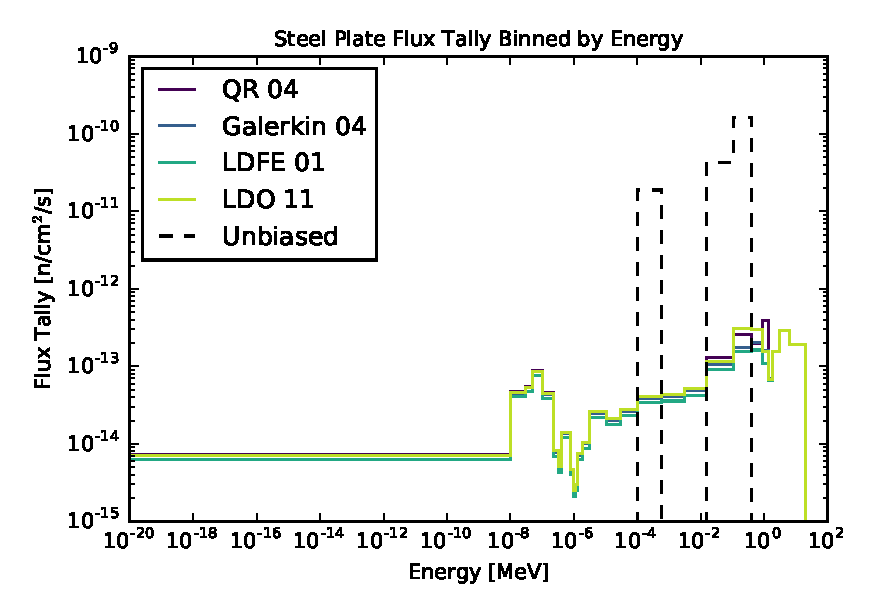
\includegraphics[max height=0.445\textheight]{img/steel-plots/mcnp/ebin-hist.eps}
\caption{Steel plate detector tally broken down by energy bin.}
\label{steel-tally-bin}
\end{figure}

\noindent This phenomenon has been 
previously documented \cite{wilsonslaybaugh} and can be largely attributed to the 
resonances in the iron cross section, shown in Figure \ref{fe-xs} with the 27n19g 
library energy group boundaries overlaid. The unresolved resonance region in the iron
cross section spans multiple energy groups, leading to inaccuracies in the discretized
multigroup cross section values used in deterministic calculations. To put this
directly in the context of the test case scenario at hand, Figure \ref{hist-xs} shows
the detector tally broken down by energy bin overlaid on the iron total cross section.
Unsurprisingly, the energy regions of large discrepancy are those in which the iron
cross section resonances lie.

\begin{figure}[!htb]
\centering
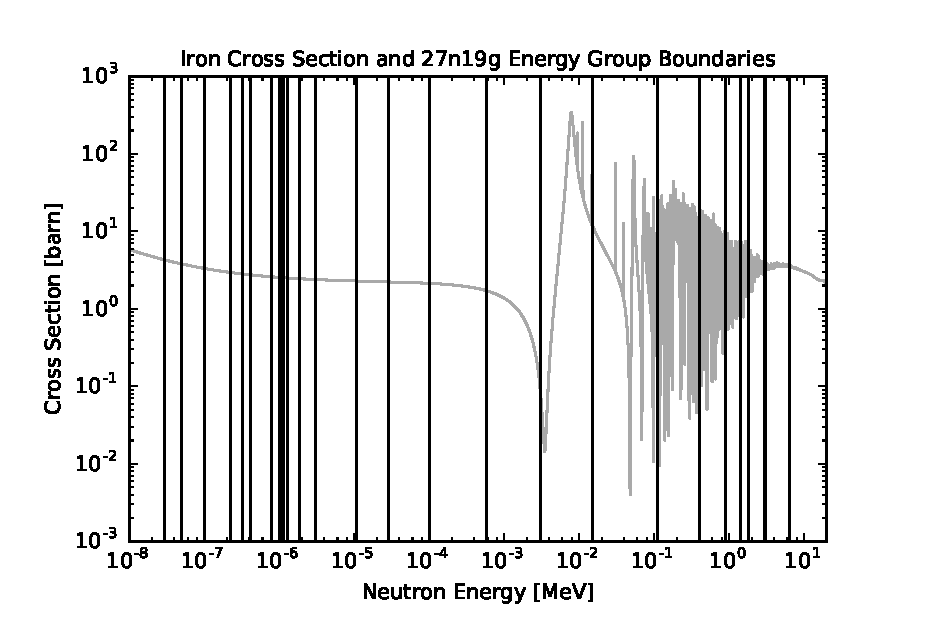
\includegraphics[max height=0.445\textheight]{img/steel-plots/fe-xs.eps}
\caption{ENDF iron total reaction cross section with 27n19g energy group limits 
         \cite{endf, advantg}.}
\label{fe-xs}
\end{figure}

\begin{figure}[!hbt]
\centering
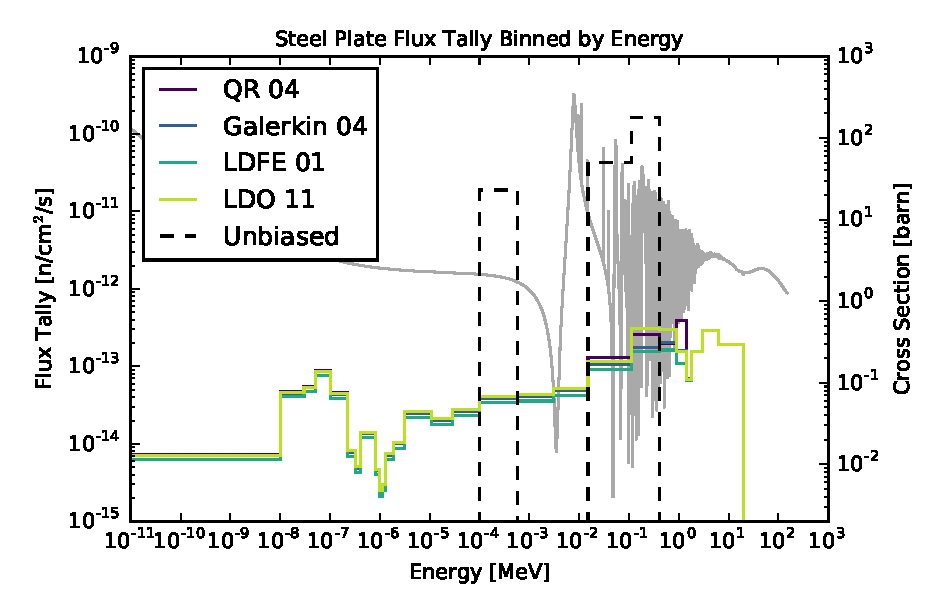
\includegraphics[max height=0.445\textheight]{img/steel-plots/mcnp/ebin-hist-xs.eps}
\caption{Steel plate detector tally broken down by energy bin with iron cross 
         section.}
\label{hist-xs}
\end{figure}

\FloatBarrier
Having explored the discrepancy between the biased and unbiased tally
results, we move on to looking at the Figures of Merit for the various Monte Carlo 
run results. Figure \ref{steel-cad-fom} shows the reported FOM value for the detector
tally for the various quadrature sets and orders. We again plot the results as a
function of angular mesh refinement with a black horizontal line denoting the FOM for
the unbiased Monte Carlo calculation. The biasing parameters corresponding to the 
LDFE quadrature set of order 1 result in the highest FOM value while those of the QR
set of order 1 result in the lowest FOM value. For all LDO quadrature sets of order 8
and above, the Figures of Merit are one order of magnitude greater than that of the
unbiased calculation.

\begin{figure}[!htb]
\centering
\includegraphics[max height=0.445\textheight]{img/steel-plots/mcnp/cadis-fom-4.eps}
\caption{FOM values for MCNP flux tally at the end of the steel plate.}
\label{steel-cad-fom}
\end{figure}

To conclude this section, we consider the overall trends in angular mesh refinement
in Figures \ref{steel-cad-tally} and \ref{steel-cad-fom}. It appears that the angular
mesh refinement does not have a great impact on the flux tally value in this scenario,
as all of the biased tally results fall within the same order of magnitude and do not
exhibit any trends as a function of the number of discrete angles used. The Figures 
of Merit vary somewhat more greatly. Specifically, the LDO biasing parameters appear
to gather around FOM values of 0.005 even as the number of discrete angles used 
is increased. So, for the steel plate in water detector tally in the context of the 
CADIS method, one could use a relatively low-order (i.e., order 8) LDO quadrature set 
to generate Monte Carlo biasing parameters that result in a Figure of Merit comparable to
(and better than most of, as seen here) those produced by finer angular meshes.

\FloatBarrier
\subsection{DLVN}

To study the DLVN problem in the context of the CADIS method, the adjoint source
was set to be the tally located at detector \#14 in the original experiment.
All of the adjoint scalar flux solutions shown in Figure \ref{dlvn-cad-adj-slices}
reflect this; the adjoint flux is highest at the specified detector location. The
differences in the adjoint scalar flux solutions shown in Figure 
\ref{dlvn-cad-adj-diff-rel} appear as ray effects from the relatively localized source
at the detector location as well as in the streaming pathway in the dog-legged void
section. Table \ref{dlvn-cad-diff-table} lists the extremal and average values of the 
relative differences between the LDO and standard quadrature results. Comparisons
between the Galerkin and LDFE quadrature sets versus the QR set are also given for
reference. On average, the LDO adjoint flux solution agrees best with the QR adjoint
flux solution with a difference of approximately 3.8\%.

\begin{table}[!hbt]
\centering
\caption{DLVN CADIS adjoint scalar flux extremal and average relative 
         differences.}
\label{dlvn-cad-diff-table}
\begin{tabular}{l|ccc}
\textbf{Comparison} & \textbf{Min. Diff.} & \textbf{Max. Diff.} & \textbf{Avg. Diff.} 
\\ \hline
LDO/QR              & 1\E{-5}             & 1.24\E{0}         & 3.78\E{-2} 
\rule{0pt}{2.6ex}   \\ 
LDO/Galerkin        & 3\E{-4}             & 5.01\E{0}         & 3.56\E{-1}          \\
LDO/LDFE            & 2\E{-5}             & 9.67\E{-1}        & 6.04\E{-2}          \\
Galerkin/QR         & 6\E{-1}             & 7.62\E{-1}        & 2.00\E{-1}          \\
LDFE/QR             & 2\E{-5}             & 3.07\E{-1}        & 5.31\E{-2}
\end{tabular}
\end{table}

\begin{figure}[!htb]
\centering
\begin{subfigure}{0.4\textwidth}
\includegraphics[max height=0.445\textheight]
{img/dlvn-plots/cad-adj/flux-qr04-slice.eps}
\subcaption{QR adjoint flux slice.}
\end{subfigure} ~
\begin{subfigure}{0.4\textwidth}
\includegraphics[max height=0.445\textheight]
{img/dlvn-plots/cad-adj/flux-gkn04-slice.eps}
\subcaption{Galerkin adjoint flux slice.}
\end{subfigure}
\\
\begin{subfigure}{0.4\textwidth}
\includegraphics[max height=0.445\textheight]
{img/dlvn-plots/cad-adj/flux-ldfe01-slice.eps}
\subcaption{LDFE adjoint flux slice.}
\end{subfigure} ~
\begin{subfigure}{0.4\textwidth}
\includegraphics[max height=0.445\textheight]
{img/dlvn-plots/cad-adj/flux-ldo11-slice.eps}
\subcaption{LDO adjoint flux slice.}
\end{subfigure}
\caption{DLVN adjoint scalar flux slices for the CADIS method.}
\label{dlvn-cad-adj-slices}
\end{figure}

\begin{figure}[!htb]
\centering
\begin{subfigure}{0.4\textwidth}
\includegraphics[max height=0.445\textheight]
{img/dlvn-plots/cad-adj/flux-diff-rel-qr04.eps}
\subcaption{LDO/QR flux rel. diff.}
\end{subfigure} ~
\begin{subfigure}{0.4\textwidth}
\includegraphics[max height=0.445\textheight]
{img/dlvn-plots/cad-adj/flux-diff-rel-gkn04.eps}
\subcaption{LDO/Galerkin flux rel. diff.}
\end{subfigure}
\\
\begin{subfigure}{0.4\textwidth}
\includegraphics[max height=0.445\textheight]
{img/dlvn-plots/cad-adj/flux-diff-rel-ldfe01.eps}
\subcaption{LDO/LDFE flux rel. diff.}
\end{subfigure}
\caption{DLVN adjoint scalar flux relative difference slices for the CADIS method.}
\label{dlvn-cad-adj-diff-rel}
\end{figure}

\clearpage
Moving forward, we look at the Monte Carlo results. For the DLVN case, 1\E{10}
neutron histories were simulated. Since the CADIS method is for one
local adjoint source, which we have set to detector \#14 here, the discussion in this
section will focus on the results for this specific detector location. Figure
\ref{dlvn-cad-tally} shows the MCNP-reported tally for the forward scalar flux at the
location of detector \#14. Here we see that all of the biased calculation values fall
within the error of the unbiased result. However, all of these tally calculations 
(biased and unbiased) do not match the experimentally calculated flux value of 
2.74\E{-7} $\pm$ 5\% n/cm$^2$/s at detector \#14.

\begin{figure}[!htb]
\centering
\includegraphics[max height=0.445\textheight]{img/dlvn-plots/mcnp/cadis-tally-14.eps}
\caption{Flux tally at detector \#14 in the DLVN problem with the CADIS method.}
\label{dlvn-cad-tally}
\end{figure}

\begin{figure}[!htb]
\centering
\includegraphics[max height=0.445\textheight]{img/dlvn-plots/mcnp/cadis-fom-14.eps}
\caption{FOM values for the DLVN problem detector \#14 tally with the CADIS 
         method.}
\label{dlvn-cad-fom}
\end{figure}

Figures \ref{dlvn-cad-tally} and \ref{dlvn-cad-fom} show similar convergence behavior 
with respect to angular mesh refinement for the biased tally calculations and Figure 
of Merit values. Beyond the lowest-order angular mesh refinement for each
quadrature type studied here, the tally result for this detector location using the
CADIS method is not impacted by further refining the angular mesh. The Figures of
Merit for the tally calculations reach a similar upper bound, but this happens more
slowly with respect to angular mesh refinement for the LDO quadrature sets. Like the
tally in the steel plate case above, the LDO quadrature set of order 8 is the optimal
choice with respect to flux tally result and FOM value for detector \#14 in the DLVN
experimental benchmark problem in the CADIS context.

\FloatBarrier
\subsection{Ispra Sodium Benchmark}
\label{sec:eurac-cad}

For these CADIS calculations, the adjoint source was set to be the detector
location farthest from the experimental neutron source. As with the previous cases, we will 
first examine the adjoint scalar flux solutions and then move on to the Monte Carlo results.
The representative LDO quadrature set used in the deterministic calculations
here is of order 9 with only 100 total angles and is
coarser than the other representative quadrature sets.

The adjoint scalar flux solutions are shown in Figure \ref{eurac-cad-slices} with
relative differences plotted in Figure \ref{eurac-cad-diff-rel} and listed in Table
\ref{eurac-cad-diff-table}. Since this
source is relatively localized in the overall problem scale, ray effects are seen in
the adjoint flux solutions as well as in the relative difference plots. For this case,
the Galerkin adjoint scalar flux matches most closely with the QR adjoint scalar flux;
a finer LDO angular mesh would likely show better agreement.

\begin{table}[!hbt]
\centering
\small
\caption{Ispra sodium test CADIS adjoint flux extremal and average relative 
         differences.}
\label{eurac-cad-diff-table}
\begin{tabular}{l|ccc}
\textbf{Comparison} & \textbf{Min. Diff.} & \textbf{Max. Diff.} & \textbf{Avg. Diff.} 
\\ \hline
LDO/QR              & 1\E{-8}             & 1.46\E{2}   & 9.71\E{-1}
\rule{0pt}{2.6ex}   \\ 
LDO/Galerkin        & 2\E{-5}             & 2.52\E{5}   & 5.74\E{2}  \\
LDO/LDFE            & 1\E{-6}             & 3.32\E{2}   & 1.28\E{0}  \\
Galerkin/QR         & 5\E{-6}             & 1.00\E{0}   & 4.62\E{-1} \\
LDFE/QR             & 6\E{-7}             & 8.10\E{1}   & 1.19\E{0}
\end{tabular}
\end{table}

\clearpage
\begin{figure}[!htb]
\begin{subfigure}{\textwidth}
\centering
\includegraphics[max height=0.445\textheight]
{img/eurac-plots/cad-adj/flux-qr04-slice.eps}
\subcaption{QR adjoint flux slice.}
\end{subfigure}
\\
\begin{subfigure}{\textwidth}
\centering
\includegraphics[max height=0.445\textheight]
{img/eurac-plots/cad-adj/flux-gkn04-slice.eps}
\subcaption{Galerkin adjoint flux slice.}
\end{subfigure}
\end{figure}
\clearpage
\begin{figure}[!htb]
\ContinuedFloat
\begin{subfigure}{\textwidth}
\centering
\includegraphics[max height=0.445\textheight]
{img/eurac-plots/cad-adj/flux-ldfe01-slice.eps}
\subcaption{LDFE adjoint flux slice.}
\end{subfigure}
\\
\begin{subfigure}{\textwidth}
\centering
\includegraphics[max height=0.445\textheight]
{img/eurac-plots/cad-adj/flux-ldo09-slice.eps}
\subcaption{LDO adjoint flux slice.}
\end{subfigure}
\caption{Ispra sodium adjoint scalar flux slices for the CADIS method.}
\label{eurac-cad-slices}
\end{figure}

\clearpage
\begin{figure}[!htb]
\begin{subfigure}{\textwidth}
\centering
\includegraphics[max height=0.445\textheight]
{img/eurac-plots/cad-adj/flux-diff-rel-qr04.eps}
\subcaption{LDO/QR flux relative difference.}
\end{subfigure}
\\
\begin{subfigure}{\textwidth}
\centering
\includegraphics[max height=0.445\textheight]
{img/eurac-plots/cad-adj/flux-diff-rel-gkn04.eps}
\subcaption{LDO/Galerkin flux relative difference.}
\end{subfigure}
\end{figure}
\clearpage
\begin{figure}[!htb]
\ContinuedFloat
\begin{subfigure}{\textwidth}
\centering
\includegraphics[max height=0.445\textheight]
{img/eurac-plots/cad-adj/flux-diff-rel-ldfe01.eps}
\subcaption{LDO/LDFE flux relative difference.}
\end{subfigure}
\caption{Ispra sodium adjoint scalar flux relative difference slices for the CADIS 
         method.}
\label{eurac-cad-diff-rel}
\end{figure}

Again, we will focus the analysis here on
the Monte Carlo results for the detector location set to be the adjoint source in the
CADIS context. Here, 1\E{9} neutron histories were simulated. 
Figure \ref{eurac-cad-tally} shows the calculated activity values for
the far detector location as a function of angular mesh refinement. All activity
values were calculated using the forward scalar flux reported by MCNP in combination
with Equation \ref{eq:act} and the data listed in Section \ref{sec:eurac-fwd}. All of
the biased results fall well within the statistical error of the unbiased calculation,
but the calculations are all four orders of magnitude greater than the experimentally
calculated activity of 0.00199 Bq/g listed in Table \ref{eurac-fwd-det}. One likely
reason for this is that the MCNP flux tallies used in these calculations include neutrons of 
all incident energies and not only those above the threshold for the \ce{^{32}S}(n,p)\ce{^{32}P}
reaction measured experimentally.

\begin{figure}[!htb]
\centering
\includegraphics[max height=0.445\textheight]{img/eurac-plots/mcnp/cadis-tally-74.eps}
\caption{Ispra sodium calculated activity in the far detector with the CADIS method.}
\label{eurac-cad-tally}
\end{figure}

\begin{figure}[!htb]
\centering
\includegraphics[max height=0.445\textheight]{img/eurac-plots/mcnp/cadis-fom-74.eps}
\caption{Ispra sodium far detector flux tally FOM values with the CADIS method.}
\label{eurac-cad-fom}
\end{figure}

Figure \ref{eurac-cad-tally} exhibits no trend for the calculated activity with
respect to angular mesh refinement; the coarsest angular mesh of each quadrature type
studied here is sufficient to achieve the same forward flux tally and calculated
activity value. The FOM values plotted in Figure \ref{eurac-cad-fom} show
differing trends for the different quadrature types. The QR biasing parameters tend
toward a Figure of Merit of approximately 1000, with the exception of those from the
quadrature set of order 4. Of the LDO quadrature sets tested here, the best
performance comes from the coarsest angular mesh, with the finest angular mesh not far
behind. So, for the Ispra sodium benchmark case in the CADIS method context, the LDO
quadrature set of order 3 would be the best one to use (of the LDO quadrature sets).

\FloatBarrier
\subsection{Simplified Portal Monitor}

To study calculations for the simplified portal monitor scenario in the context of the CADIS 
method, the adjoint source was set to be the top detector in the small array. The adjoint scalar
flux solutions are plotted in Figure \ref{cargo-cad-adj-slices}. Ray effects appear
drastically in all of the adjoint scalar flux solutions. Figure \ref{cargo-cad-gkn}
shows regions where the adjoint scalar flux solution is negative for the 
representative Galerkin quadrature set; these regions are plotted in white.
Because of these negative flux regions, Table \ref{cargo-cad-diff-table} shows the 
extremal values of the magnitudes of the relative flux differences, calculated as

\begin{equation}
\phi_{\mathrm{diff}} = 
\frac{\left|\phi_{\mathrm{LDO}}-\phi_{\mathrm{ref}}\right|}{\left|\phi_{\mathrm{ref}}\right|}.
\label{flux-diff-gkn}
\end{equation}

\noindent All of the flux solutions show poor agreement, likely because of the localized source
and streaming paths created by this scenario's materials and geometry. Still, the LDO adjoint
scalar flux solution agrees with the QR adjoint scalar flux solution better than the Galerkin
or LDFE solutions, on average.

\begin{table}[!hbt]
\centering
\caption{Portal monitor CADIS adjoint scalar flux extremal and average relative 
         differences.}
\label{cargo-cad-diff-table}
\begin{tabular}{l|ccc}
\textbf{Comparison} & \textbf{Min. Diff.} & \textbf{Max. Diff.} & \textbf{Avg. Diff.} 
\\ \hline
LDO/QR              & 2\E{-4}             & 1.83\E{2}    & 2.27\E{0}
\rule{0pt}{2.6ex}   \\ 
LDO/Galerkin        & 1\E{-4}             & 6.20\E{4}    & 4.29\E{1}  \\
LDO/LDFE            & 2\E{-4}             & 2.54\E{2}    & 3.46\E{0}   \\
Galerkin/QR         & 1\E{-3}             & 2.59\E{2}    & 3.81\E{0}   \\
LDFE/QR             & 6\E{-5}             & 6.48\E{1}    & 2.21\E{0}
\end{tabular}
\end{table}

\clearpage
\begin{figure}[!htb]
\begin{subfigure}{\textwidth}
\centering
\includegraphics[max height=0.445\textheight]
{img/cargo-plots/cad-adj/flux-qr04-slice.eps}
\subcaption{QR adjoint flux slice.}
\end{subfigure}
\\
\begin{subfigure}{\textwidth}
\centering
\includegraphics[max height=0.445\textheight]
{img/cargo-plots/cad-adj/flux-gkn04-slice.eps}
\subcaption{Galerkin adjoint flux slice.}
\label{cargo-cad-gkn}
\end{subfigure}
\end{figure}
\clearpage
\begin{figure}[!htb]
\ContinuedFloat
\begin{subfigure}{\textwidth}
\centering
\includegraphics[max height=0.445\textheight]
{img/cargo-plots/cad-adj/flux-ldfe01-slice.eps}
\subcaption{LDFE adjoint flux slice.}
\end{subfigure}
\\
\begin{subfigure}{\textwidth}
\centering
\includegraphics[max height=0.445\textheight]
{img/cargo-plots/cad-adj/flux-ldo11-slice.eps}
\subcaption{LDO adjoint flux slice.}
\end{subfigure}
\caption{Simplified portal monitor adjoint scalar flux slices for the CADIS method.}
\label{cargo-cad-adj-slices}
\end{figure}

\clearpage
\begin{figure}[!htb]
\begin{subfigure}{\textwidth}
\centering
\includegraphics[max height=0.445\textheight]
{img/cargo-plots/cad-adj/flux-diff-rel-qr04.eps}
\subcaption{LDO/QR flux relative difference.}
\end{subfigure}
\\
\begin{subfigure}{\textwidth}
\centering
\includegraphics[max height=0.445\textheight]
{img/cargo-plots/cad-adj/flux-diff-rel-gkn04.eps}
\subcaption{LDO/Galerkin flux relative difference.}
\end{subfigure}
\end{figure}
\clearpage
\begin{figure}[!htb]
\ContinuedFloat
\begin{subfigure}{\textwidth}
\centering
\includegraphics[max height=0.445\textheight]
{img/cargo-plots/cad-adj/flux-diff-rel-ldfe01.eps}
\subcaption{LDO/LDFE flux relative difference.}
\end{subfigure}
\caption{Portal monitor adjoint scalar flux relative difference slices for the CADIS 
         method.}
\label{cargo-cad-adj-diff-rel}
\end{figure}

Finally, we move on to the results and analysis of the Monte Carlo calculations, in which
1\E{9} particle histories were simulated.
Again, since the CADIS adjoint source was set to be the top detector location, we
focus the discussion in this section on the results for that specific location.
Figures \ref{cargo-cad-tally} and \ref{cargo-cad-fom} show the MCNP-reported forward scalar 
flux tally values and Figures of Merit, respectively. As with the other test cases, the
values are plotted as a function of the number of quadrature points used to generate
the biasing parameters in order to explore the impact of angular mesh refinement on
flux tally and FOM.

\begin{figure}[!htb]
\centering
\includegraphics[max height=0.445\textheight]{img/cargo-plots/mcnp/cadis-tally-14.eps}
\caption{Flux tally in the portal monitor top detector using the CADIS method.}
\label{cargo-cad-tally}
\end{figure}

\begin{figure}[!htb]
\centering
\includegraphics[max height=0.445\textheight]{img/cargo-plots/mcnp/cadis-fom-14.eps}
\caption{CADIS method FOM values for the portal monitor top detector flux tally.}
\label{cargo-cad-fom}
\end{figure}

Similar to other test cases, the flux tally values reported in Figure 
\ref{cargo-cad-tally} show a trend of converging to a stable value after the first few
coarsest angular meshes. The flux tally values from the biased calculations all fall
within the statistical error of that of the unbiased calculation but appear to require
a minimum value of approximately 100 discrete angular values in order to stabilize.
Figure \ref{cargo-cad-fom} shows a strong correlation between the number of quadrature
points and the flux tally FOM, eventually approaching an upper limit around 100.
The LDO Figures of Merit increase most rapidly with the
number of quadrature points used, so one would want to use a higher-order LDO 
quadrature set to generate Monte Carlo biasing parameters.

\FloatBarrier
\subsection{Summary}

In this section, we examined the deterministic and Monte Carlo results for the four
test case scenarios in the context of the CADIS method. 
For all of the test cases, little correlation was noted between angular mesh
refinement and MCNP-reported forward flux tally value beyond the suggestion to use
at least 100 discrete angles for the simplified portal monitor scenario. The reported
FOM values also exhibited minimal correlation with angular mesh refinement except in
the case of the portal monitor scenario, where the flux tally FOM increased with angular mesh
refinement while approaching an upper limit.

For the three test cases in which neutrons were transported, the LDO quadrature sets 
of lower orders (3 and 8) were the most effective of the LDO sets for both flux tally
value and FOM achievement. That is, if one were interested in using an LDO quadrature
set to generate Monte Carlo biasing parameters for a given neutron transport problem
in the context of the CADIS method, we would suggest performing the deterministic
calculation with an LDO quadrature set of order 8. For a photon transport problem
considered in the CADIS context, we would suggest the finest available LDO quadrature
set, based on the results seen here.

\FloatBarrier
\section{FW-CADIS Calculations}

Finally, we examine the performance of the various quadrature types in the context of
the \fwc\ method. Similar to the analysis for the CADIS method, we will first look at 
the deterministic adjoint scalar flux solutions from the representative quadrature 
sets to compare the calculations using the LDO equations versus the standard 
quadrature types. Recalling Section \ref{sec:fwcadis}, the \fwc\ method incorporates 
both forward and adjoint scalar flux solutions. Because the adjoint source may be
specified differently between the CADIS and \fwc\ methods, it is instructive to look
at the \fwc\ deterministic adjoint scalar flux solutions. However, the deterministic
forward flux solutions used in the \fwc\ method are the same as those discussed
in Section \ref{sec:det-fwd} and so we will not repeat the analysis here. Lastly, we
again look at result metrics from the various Monte Carlo runs to compare the variance
reduction parameter generation efficacy of the different quadrature types.

\subsection{Steel Plate in Water}

For the \fwc\ calculations for the steel plate in water, the adjoint source was set to
be a mesh tally over all of the air beyond the steel plate. The discretization for the
adjoint source mesh tally is the same as that listed in 
Section \ref{sec:steel_params}. Specifically, the adjoint source mesh is identical to
the overall problem mesh in the $x-$ and $y-$directions but starts at $z = 130$ cm and
extends to the problem boundary at $z = 140$ cm.

Figure \ref{steel-fwc-adj-slices} shows the adjoint scalar flux solutions for the
representative quadrature sets for the steel plate embedded in water. As expected, in
each solution, the adjoint flux is highest in the chosen adjoint source region for the
problem and decreases logarithmically in the $z-$direction. Table 
\ref{steel-fwc-diff-table} lists the minimum, maximum, and average relative adjoint
scalar flux solution differences for the comparisons plotted in Figure 
\ref{steel-fwc-adj-diff-rel}. As with earlier cases, the Galerkin/QR and LDFE/QR
comparisons are also tabulated for reference. Like other deterministic flux
comparisons for the steel plate embedded in water, the LDO flux solution best matches
the QR flux solution, with an average relative difference of 4.6\% for the \fwc\ adjoint
scalar flux.

\begin{table}[!hbt]
\centering
\caption{Steel plate \fwc\ adjoint scalar flux extremal and average relative 
         differences.}
\label{steel-fwc-diff-table}
\begin{tabular}{l|ccc}
\textbf{Comparison} & \textbf{Min. Diff.} & \textbf{Max. Diff.} & \textbf{Avg. Diff.} 
\\ \hline
LDO/QR              & 2\E{-4}             & 1.66\E{-1}    & 4.63\E{-2}
\rule{0pt}{2.6ex}   \\ 
LDO/Galerkin        & 2\E{-5}             & 1.85\E{0}     & 7.16\E{-1}      \\
LDO/LDFE            & 8\E{-2}             & 2.41\E{-1}    & 1.92\E{-1}      \\
Galerkin/QR         & 5\E{-4}             & 5.98\E{0}     & 2.85\E{0}      \\
LDFE/QR             & 3\E{-2}             & 3.37\E{-1}    & 2.09\E{-1}
\end{tabular}
\end{table}

\noindent Comparing Figure \ref{steel-fwc-adj-diff-rel} with Figure 
\ref{steel-cad-adj-diff-rel}, we see that the relative differences among the \fwc\ adjoint
scalar flux solutions are more uniform than those of the CADIS adjoint flux solutions. This is
to be expected, as the CADIS adjoint source is much more localized than the \fwc\ for the
steel plate scenario studies conducted here.

\begin{figure}[!htb]
\centering
\begin{subfigure}{0.4\textwidth}
\includegraphics[max height=0.445\textheight]
{img/steel-plots/fwc-adj/flux-qr04-slice.eps}
\subcaption{QR adjoint flux slice.}
\end{subfigure} ~
\begin{subfigure}{0.4\textwidth}
\includegraphics[max height=0.445\textheight]
{img/steel-plots/fwc-adj/flux-gkn04-slice.eps}
\subcaption{Galerkin adjoint flux slice.}
\end{subfigure}
\\
\begin{subfigure}{0.4\textwidth}
\includegraphics[max height=0.445\textheight]
{img/steel-plots/fwc-adj/flux-ldfe01-slice.eps}
\subcaption{LDFE adjoint flux slice.}
\end{subfigure} ~
\begin{subfigure}{0.4\textwidth}
\includegraphics[max height=0.445\textheight]
{img/steel-plots/fwc-adj/flux-ldo11-slice.eps}
\subcaption{LDO adjoint flux slice.}
\end{subfigure}
\caption{Steel plate adjoint scalar flux slices for the \fwc\ method.}
\label{steel-fwc-adj-slices}
\end{figure}

\begin{figure}[!htb]
\centering
\begin{subfigure}{0.4\textwidth}
\includegraphics[max height=0.445\textheight]
{img/steel-plots/fwc-adj/flux-diff-rel-qr04.eps}
\subcaption{LDO/QR flux rel. diff.}
\end{subfigure} ~
\begin{subfigure}{0.4\textwidth}
\includegraphics[max height=0.445\textheight]
{img/steel-plots/fwc-adj/flux-diff-rel-gkn04.eps}
\subcaption{LDO/Galerkin flux rel. diff.}
\end{subfigure}
\\
\begin{subfigure}{0.4\textwidth}
\includegraphics[max height=0.445\textheight]
{img/steel-plots/fwc-adj/flux-diff-rel-ldfe01.eps}
\subcaption{LDO/LDFE flux rel. diff.}
\end{subfigure}
\caption{Steel plate adjoint flux relative difference slices for the \fwc\
         method.}
\label{steel-fwc-adj-diff-rel}
\end{figure}

\clearpage
Next, we will look at the results for the mesh tally in the air region of the 
scenario. The Monte Carlo run with biasing parameters from the Galerkin quadrature 
set of order 2 was not able to finish in a timely manner for the hardware
configuration used in this work, so Monte Carlo results for this data point are not
included here. The calculations for this test case scenario used 1\E{9} neutron histories.

Figure \ref{steel-fwc-tally} shows the total tally summed over all air in the
problem for the biased and unbiased calculations. The biased calculations are plotted
as a function of angular mesh refinement and the unbiased calculation value is shown
as a black horizontal line. Like the CADIS method, the \fwc\ method generates biasing
parameters such that the biased Monte Carlo flux tally results all fall far below that
of the unbiased calculation. Similarly, in this case, the angular mesh refinement has
little impact on the tally result. So, if using an LDO quadrature set to generate
biasing parameters with the \fwc\ method in a similar scenario, a low-order LDO
angular mesh could be used to good effect.

\begin{figure}[!htb]
\centering
\includegraphics[max height=0.445\textheight]{img/steel-plots/mcnp/fwc-tally.eps}
\caption{Flux tally over the air region in the steel plate test with the \fwc\ method.}
\label{steel-fwc-tally}
\end{figure}

To analyze the performance of the representative quadrature sets' variance reduction
parameters for the steel plate in water case using the \fwc\ method, we will look at
the average FOM values over the entire adjoint source mesh tally. The Figures of
Merit were calculated by taking the average relative error over all spatial cells in the
air block mesh tally and using that mean value in combination with the MCNP-reported 
computer time and Equation \ref{eq:fom}. Figure \ref{steel-fwc-fom} shows these
average Figures of Merit as a function of the number of angles used in generating the
biasing parameters. The average FOM for the unbiased calculation is shown as a
horizontal black line.

\begin{figure}[!htb]
\centering
\includegraphics[max height=0.445\textheight]{img/steel-plots/mcnp/fwcadis-fom.eps}
\caption{Average FOM values for the mesh tally in the \fwc\ steel plate scenario.}
\label{steel-fwc-fom}
\end{figure}

We see a different trend here in that the highest average FOM values tend to come from
quadrature sets with mid-range angular mesh refinement; the coarsest and finest
angular meshes produce Monte Carlo biasing parameters that result in reduced Figures
of Merit. Considering Figures \ref{steel-fwc-tally} and \ref{steel-fwc-fom}, we note
that one would wish to use a lower-order (e.g., order 5) LDO quadrature set to generate
variance reduction parameters for a Monte Carlo mesh tally using the \fwc\ method.

\FloatBarrier
\subsection{DLVN}

Considering the DLVN case with the \fwc\ method, the adjoint source was specified to
be the combination of all of the detector locations in the problem. In accordance 
with this, the adjoint scalar flux solutions shown in Figure \ref{dlvn-fwc-adj-slices}
demonstrate the highest source values in the region where four out of the six
detector locations are concentrated. Figure \ref{dlvn-fwc-adj-diff-rel} displays the
relative differences between the LDO adjoint scalar flux solution and those of
the three standard quadrature types with extremal and average relative difference
values listed in Table \ref{dlvn-fwc-diff-table}. 
Of the standard quadrature types, the LDO adjoint flux solution differs the least from the QR
adjoint flux solution, with an average relative difference of about 11\% for this \fwc\ adjoint
source specification for the DLVN problem. Given the more spatially 
generalized source specification, it is unsurprising to see uniform differences in 
Figures \ref{dlvn-fwc-qr-ldo} and \ref{dlvn-fwc-ldfe-ldo}. The nonuniform differences 
in Figure \ref{dlvn-fwc-gkn-ldo} may be attributed to the relative coarseness of the
representative Galerkin quadrature set.

\begin{table}[!hbt]
\centering
\caption{DLVN \fwc\ adjoint scalar flux extremal and average relative differences.}
\label{dlvn-fwc-diff-table}
\begin{tabular}{l|ccc}
\textbf{Comparison} & \textbf{Min. Diff.} & \textbf{Max. Diff.} & \textbf{Avg. Diff.} 
\\ \hline
LDO/QR              & 1\E{-3}             & 4.32\E{-1} & 1.12\E{-1}
\rule{0pt}{2.6ex}   \\ 
LDO/Galerkin        & 2\E{-5}             & 1.90\E{0}  & 1.79\E{-1}      \\
LDO/LDFE            & 1\E{-2}             & 3.97\E{-1} & 1.73\E{-1}      \\
Galerkin/QR         & 2\E{-4}             & 6.88\E{-1} & 2.68\E{-1}      \\
LDFE/QR             & 4\E{-4}             & 2.58\E{-1} & 5.42\E{-2}
\end{tabular}
\end{table}

\begin{figure}[!htb]
\centering
\begin{subfigure}{0.4\textwidth}
\includegraphics[max height=0.445\textheight]
{img/dlvn-plots/fwc-adj/flux-qr04-slice.eps}
\subcaption{QR adjoint flux slice.}
\end{subfigure} ~
\begin{subfigure}{0.4\textwidth}
\includegraphics[max height=0.445\textheight]
{img/dlvn-plots/fwc-adj/flux-gkn04-slice.eps}
\subcaption{Galerkin adjoint flux slice.}
\end{subfigure}
\\
\begin{subfigure}{0.4\textwidth}
\includegraphics[max height=0.445\textheight]
{img/dlvn-plots/fwc-adj/flux-ldfe01-slice.eps}
\subcaption{LDFE adjoint flux slice.}
\end{subfigure} ~
\begin{subfigure}{0.4\textwidth}
\includegraphics[max height=0.445\textheight]
{img/dlvn-plots/fwc-adj/flux-ldo11-slice.eps}
\subcaption{LDO adjoint flux slice.}
\end{subfigure}
\caption{DLVN adjoint scalar flux slices for the \fwc\ method.}
\label{dlvn-fwc-adj-slices}
\end{figure}

\begin{figure}[!htb]
\centering
\begin{subfigure}{0.4\textwidth}
\includegraphics[max height=0.445\textheight]
{img/dlvn-plots/fwc-adj/flux-diff-rel-qr04.eps}
\subcaption{LDO/QR flux rel. diff.}
\label{dlvn-fwc-qr-ldo}
\end{subfigure} ~
\begin{subfigure}{0.4\textwidth}
\includegraphics[max height=0.445\textheight]
{img/dlvn-plots/fwc-adj/flux-diff-rel-gkn04.eps}
\subcaption{LDO/Galerkin flux rel. diff.}
\label{dlvn-fwc-gkn-ldo}
\end{subfigure}
\\
\begin{subfigure}{0.4\textwidth}
\includegraphics[max height=0.445\textheight]
{img/dlvn-plots/fwc-adj/flux-diff-rel-ldfe01.eps}
\subcaption{LDO/LDFE flux rel. diff.}
\label{dlvn-fwc-ldfe-ldo}
\end{subfigure}
\caption{DLVN adjoint scalar flux relative difference slices for the \fwc\ method.}
\label{dlvn-fwc-adj-diff-rel}
\end{figure}

\clearpage
Moving on to the Monte Carlo results and analysis, we look at the flux tallies and 
Figures of Merit for all of the detector locations in the DLVN experimental benchmark.
Recall that 1\E{10} particle histories were simulated.
Figure \ref{dlvn-fwc-tally} shows all of the detector locations' MCNP-reported forward scalar
flux tallies plotted as a function of angular mesh refinement used to generate biasing 
parameters in addition to the Figures of Merit for the flux tallies.
In each plot, the unbiased flux tally result is shown as a horizontal black line.

Figures \ref{dlvn-fwc-5} and \ref{dlvn-fwc-9} exhibit the same lack of trend in flux tally as a
function of angular mesh refinement. That is, in general, for detector locations \#5 and \#9,
using more discrete angles in the \fwc\ deterministic calculations does not greatly impact the
flux tally result from MCNP. Figures \ref{dlvn-fwc-13} and \ref{dlvn-fwc-14} show similar
behavior with the exception of the most coarse angular meshes. For these detector locations, any
angular mesh refinement other than the coarsest angular mesh will produce a consistent forward 
scalar flux tally result. Figures \ref{dlvn-fwc-11} and \ref{dlvn-fwc-12} show slightly more
variation in flux tally result with angular mesh refinement. These two detector locations' 
tallies have also higher statistical error relative to those at the other detector locations. 
Overall, though, the flux tallies at detectors \#11 and \#12 are not heavily impacted by the
refinement of the angular mesh used in generating the Monte Carlo biasing parameters, but
a mid-range number of quadrature points should be used to avoid the large statistical
errors seen at the extreme ends of the angular mesh refinement spectrum.

Like their corresponding flux tally graphs, Figures \ref{dlvn-fwc-5}, \ref{dlvn-fwc-9}, and
\ref{dlvn-fwc-13} show almost no variation in FOM with angular mesh refinement for the tallies
at detector locations \#5, \#9, and \#13. This is to be expected, considering the uniform
statistical error and stable flux tally results at these locations. Figure \ref{dlvn-fwc-11}
shows variation in FOM with angular mesh refinement that is more varied, which corresponds to
the larger statistical uncertainties in the flux tally values for detector \#11. Figure
\ref{dlvn-fwc-12} shows little variation in FOM with angular mesh refinement with the 
exception of the finest QR set. Lastly, \ref{dlvn-fwc-14} shows an upper FOM limit of 
approximately 200 across all quadrature types, with the Figure of Merit largely consistent
across quadrature types with the exception of QR angular meshes.

In Table \ref{dlvn-fwc-det} we compare the Monte Carlo forward flux tally results for the 
representative quadrature sets listed in Section \ref{params}. Results from the unbiased Monte 
Carlo calculation are also included for comparison. All Monte Carlo
flux tally values are reported with an uncertainty of one standard deviation. For all detector
locations, the Monte Carlo flux tallies do not match the experimentally measured flux values for
any of the representative quadrature sets or the unbiased calculation, so we only compare the
Monte Carlo calculations in this table. We do note that the Monte Carlo calculations
overestimate the flux tally at all detector locations with the exception of detector \#13.
The flux tallies at detectors 5, 9, 13, and 14 all match within statistical uncertainty for all
of the Monte Carlo calculations. At detector \#11, the biased Monte Carlo calculations match
within standard error, but the calculations using the QR and LDO biasing parameter fall outside
of the error bounds of the unbiased calculation. Somewhat similarly, at detector \#14, all of
the biased calculations match one another within statistical uncertainty, but they are all
outside of the error bounds of the unbiased flux tally calculation.

\begin{table}[!htb]
\centering
\footnotesize
\caption{DLVN benchmark flux tallies [n/cm$^2$/s] calculated with \fwc.}
\label{dlvn-fwc-det}
\begin{tabular}{l|ccccc}
         & \textbf{QR} & \textbf{Galerkin} & \textbf{LDFE} 
         & \textbf{LDO} & \textbf{Unbiased}  \\ \hline
 Det. \#5 & \mr{1.3341 $\pm$ 0.0003} & \mr{1.3344 $\pm$ 0.0003} & \mr{1.3347 $\pm$ 0.0004} &
            \mr{1.3344 $\pm$ 0.0003} & \mr{1.3315 $\pm$ 0.0092} \rule{0pt}{2.6ex} \\
    (\E{-7})      &    &   &  &   &    \\
 Det. \#9 & \mr{2.5225 $\pm$ 0.0005} & \mr{2.5224 $\pm$ 0.0005} & \mr{2.5229 $\pm$ 0.0004} &
            \mr{2.2555 $\pm$ 0.0004} & \mr{2.5104 $\pm$ 0.0127} \rule{0pt}{2.6ex}  \\
   (\E{-7}) &   &  &  &  &   \\
 Det. \#11 & \mr{1.4420 $\pm$ 0.0005} & \mr{1.4451 $\pm$ 0.0027} & \mr{1.4446 $\pm$ 0.0026} &
            \mr{1.4463 $\pm$ 0.0015} & \mr{1.4463 $\pm$ 0.0010} \rule{0pt}{2.6ex} \\
   (\E{-5}) &   &  &  &  &   \\
 Det. \#12 & \mr{2.4749 $\pm$ 0.0004} & \mr{2.4743 $\pm$ 0.0004} & \mr{2.4751 $\pm$ 0.0004} &
            \mr{2.4744 $\pm$ 0.0004} & \mr{2.4684 $\pm$ 0.0042}  \rule{0pt}{2.6ex} \\
    (\E{-6}) &   &  &  &  &   \\
 Det. \#13 & \mr{4.3984 $\pm$ 0.0011} & \mr{4.3997 $\pm$ 0.0011} & \mr{4.3994 $\pm$ 0.0011} &
            \mr{4.3983 $\pm$ 0.0011} & \mr{4.4170 $\pm$ 0.0175}  \rule{0pt}{2.6ex} \\
    (\E{-7}) &   &  &  &  &   \\
 Det. \#14 & \mr{7.0070 $\pm$ 0.0025} & \mr{7.0829 $\pm$ 0.0045} & \mr{7.0813 $\pm$ 0.0026} &
            \mr{7.0834 $\pm$ 0.0032} & \mr{7.0694 $\pm$ 0.0216}  \rule{0pt}{2.6ex} \\
    (\E{-7}) &   &  &  &  &   \\ \hline
\end{tabular}
\end{table}

To examine the FOM values in a more quantifiable way, Table \ref{dlvn-fwc-fom-table} lists the
FOM values for all detector locations for each of the representative quadrature sets as well as
the unbiased calculation. The maximum FOM value at each detector location is emphasized.
Of the six detector locations, the LDO quadrature set achieves the highest FOM
for two of the locations. The QR quadrature set is the only other type to also
deliver the highest FOM for two out of six detectors; the Galerkin and LDFE
quadrature set biasing parameters each only achieve the highest FOM at one detector.
So, the LDO quadrature set's biasing parameters perform comparably
to those from the QR quadrature set with respect to obtaining high FOM values
for multiple detector locations using the \fwc\ method for the DLVN problem.

\begin{table}[!hbt]
\centering
\caption{\fwc\ FOM values for representative quadratures for the DLVN problem.}
\label{dlvn-fwc-fom-table}
\begin{tabular}{l|cccccc}
\multicolumn{1}{l|}{Quad. Type}
& \multicolumn{1}{l}{Det. \#5}
& \multicolumn{1}{l}{Det. \#9}
& \multicolumn{1}{l}{Det. \#11}
& \multicolumn{1}{l}{Det. \#12}
& \multicolumn{1}{l}{Det. \#13}
& \multicolumn{1}{l}{Det. \#14}
\\ \hline
\begin{tabular}[c]{@{}l@{}}   QR \end{tabular} 
& \begin{tabular}[c]{@{}c@{}} 483.01 \end{tabular} % fom for #5
& \begin{tabular}[c]{@{}c@{}} 709.51 \end{tabular} % fom for #9
& \begin{tabular}[c]{@{}c@{}} \textbf{202.66} \end{tabular} % fom for #11
& \begin{tabular}[c]{@{}c@{}} 747.91 \end{tabular} % fom for #12
& \begin{tabular}[c]{@{}c@{}} 380.84 \end{tabular} % fom for #13
& \begin{tabular}[c]{@{}c@{}} \textbf{185.40} \end{tabular} % fom for #14
\\
\begin{tabular}[c]{@{}l@{}}   Galerkin \end{tabular} 
& \begin{tabular}[c]{@{}c@{}} \textbf{527.79} \end{tabular} % fom for #5
& \begin{tabular}[c]{@{}c@{}} 649.88 \end{tabular} % fom for #9
& \begin{tabular}[c]{@{}c@{}} 5.9934 \end{tabular} % fom for #11
& \begin{tabular}[c]{@{}c@{}} 798.88 \end{tabular} % fom for #12
& \begin{tabular}[c]{@{}c@{}} 326.11 \end{tabular} % fom for #13
& \begin{tabular}[c]{@{}c@{}} 52.098 \end{tabular} % fom for #14
\\
\begin{tabular}[c]{@{}l@{}}   LDFE \end{tabular} 
& \begin{tabular}[c]{@{}c@{}} 310.28 \end{tabular} % fom for #5
& \begin{tabular}[c]{@{}c@{}} 710.43 \end{tabular} % fom for #9
& \begin{tabular}[c]{@{}c@{}} 6.6749 \end{tabular} % fom for #11
& \begin{tabular}[c]{@{}c@{}} 926.28 \end{tabular} % fom for #12
& \begin{tabular}[c]{@{}c@{}} \textbf{391.62} \end{tabular} % fom for #13
& \begin{tabular}[c]{@{}c@{}} 166.51 \end{tabular} % fom for #14
\\
\begin{tabular}[c]{@{}l@{}}   LDO \end{tabular}
& \begin{tabular}[c]{@{}c@{}} 478.24 \end{tabular} % fom for #5
& \begin{tabular}[c]{@{}c@{}} \textbf{721.22} \end{tabular} % fom for #9
& \begin{tabular}[c]{@{}c@{}} 19.959 \end{tabular} % fom for #11
& \begin{tabular}[c]{@{}c@{}} \textbf{943.96} \end{tabular} % fom for #12
& \begin{tabular}[c]{@{}c@{}} 369.42 \end{tabular} % fom for #13
& \begin{tabular}[c]{@{}c@{}} 110.40 \end{tabular} % fom for #14
\\
Unbiased  & 0.14912 & 0.27845 & 14.555 & 2.5256 & 0.45376 & 0.76362
\end{tabular}
\end{table}

In summary, for test case scenarios such as the DLVN problem in which the \fwc\ method is used
to generate Monte Carlo variance reduction parameters to optimize the response at multiple
flux tally detector locations, a relatively coarse quadrature set of any of the types studied
here can be used to sufficient effect. However, the coarsest available quadrature sets should
be avoided; flux tally results and Figures of Merit for the various detector locations tend to
level out as a function of angular mesh refinement beyond the quadrature sets with the fewest
number of angles. In particular, if using an LDO quadrature set in another similar scenario, we
would suggest using a point set of order 5 or 8.

\begin{figure}[!htb]
\begin{subfigure}{\linewidth}
\centering
\includegraphics[max height=0.445\textheight]
{img/dlvn-plots/mcnp/fwc-5.eps}
\subcaption{MCNP-reported forward flux tally and FOM values at detector \#5.}
\label{dlvn-fwc-5}
\end{subfigure} 
\\
\begin{subfigure}{\linewidth}
\centering
\includegraphics[max height=0.445\textheight]
{img/dlvn-plots/mcnp/fwc-9.eps}
\subcaption{MCNP-reported forward flux tally and FOM values at detector \#9.}
\label{dlvn-fwc-9}
\end{subfigure}
\end{figure}
\clearpage
\begin{figure}[!htb]
\ContinuedFloat
\begin{subfigure}{\linewidth}
\centering
\includegraphics[max height=0.445\textheight]
{img/dlvn-plots/mcnp/fwc-11.eps}
\subcaption{MCNP-reported forward flux tally and FOM values at detector \#11.}
\label{dlvn-fwc-11}
\end{subfigure}
\\
\begin{subfigure}{\linewidth}
\centering
\includegraphics[max height=0.445\textheight]
{img/dlvn-plots/mcnp/fwc-12.eps}
\subcaption{MCNP-reported forward flux tally and FOM values at detector \#12.}
\label{dlvn-fwc-12}
\end{subfigure}
\end{figure}
\clearpage
\begin{figure}[!htb]
\ContinuedFloat
\begin{subfigure}{\linewidth}
\centering
\includegraphics[max height=0.445\textheight]
{img/dlvn-plots/mcnp/fwc-13.eps}
\subcaption{MCNP-reported forward flux tally and FOM values at detector \#13.}
\label{dlvn-fwc-13}
\end{subfigure} 
\\
\begin{subfigure}{\linewidth}
\centering
\includegraphics[max height=0.445\textheight]
{img/dlvn-plots/mcnp/fwc-14.eps}
\subcaption{MCNP-reported forward flux tally and FOM values at detector \#14.}
\label{dlvn-fwc-14}
\end{subfigure}
\caption{\fwc\ flux tallies and FOM values for the DLVN problem.}
\label{dlvn-fwc-tally}
\end{figure}

\FloatBarrier
\subsection{Ispra Sodium Benchmark}

As in the previous case, the adjoint source for the Ispra sodium benchmark problem in
the context of the \fwc\ method was specified to be the combination of all of the 
detector locations in the problem. Figure \ref{eurac-fwc-slices} shows the adjoint scalar
flux solutions for the representative quadrature sets based on this specification. Relative
differences between the representative LDO adjoint scalar flux and the standard quadratures'
adjoint scalar fluxes are shown in Figure \ref{eurac-fwc-diff-rel} with minimum, maximum, and
average relative differences listed in Table \ref{eurac-fwc-diff-table}. Again, comparisons of
the QR flux solution against the Galerkin and LDFE flux solutions are tabulated for reference
as well.

\begin{table}[!hbt]
\centering
\caption{Ispra sodium \fwc\ adjoint flux extremal and average relative differences.}
\label{eurac-fwc-diff-table}
\begin{tabular}{l|ccc}
\textbf{Comparison} & \textbf{Min. Diff.} & \textbf{Max. Diff.} & \textbf{Avg. Diff.} 
\\ \hline
LDO/QR              & 2\E{-6}             & 4.40\E{1}       & 5.93\E{-1}
\rule{0pt}{2.6ex}   \\  
LDO/Galerkin        & 6\E{-7}             & 4.45\E{4}       & 1.63\E{2}   \\
LDO/LDFE            & 1\E{-6}             & 1.30\E{2}       & 7.42\E{-1}  \\
Galerkin/QR         & 2\E{-6}             & 1.00\E{0}       & 4.42\E{-1}  \\
LDFE/QR             & 3\E{-6}             & 5.05\E{1}       & 8.00\E{-1}
\end{tabular}
\end{table}

\noindent Comparing these differences to the values listed in Table \ref{eurac-cad-diff-table},
we see that the LDO adjoint flux matches those of the standard quadratures more closely on
average in the \fwc\ method than the CADIS method. This is to be expected, as the adjoint source
in the \fwc\ method is much less localized than in the CADIS method for this scenario. As with 
the forward and CADIS adjoint flux comparisons for the Ispra sodium benchmark, the differences 
between the representative LDO flux solution and the representative standard quadratures' flux
solutions are exacerbated by the relatively coarse LDO angular mesh.

\clearpage
\begin{figure}[!htb]
\begin{subfigure}{\textwidth}
\centering
\includegraphics[max height=0.445\textheight]
{img/eurac-plots/fwc-adj/flux-qr04-slice.eps}
\subcaption{QR adjoint flux slice.}
\end{subfigure}
\\
\begin{subfigure}{\textwidth}
\centering
\includegraphics[max height=0.445\textheight]
{img/eurac-plots/fwc-adj/flux-gkn04-slice.eps}
\subcaption{Galerkin adjoint flux slice.}
\end{subfigure}
\end{figure}
\clearpage
\begin{figure}[!htb]
\ContinuedFloat
\begin{subfigure}{\textwidth}
\centering
\includegraphics[max height=0.445\textheight]
{img/eurac-plots/fwc-adj/flux-ldfe01-slice.eps}
\subcaption{LDFE adjoint flux slice.}
\end{subfigure}
\\
\begin{subfigure}{\textwidth}
\centering
\includegraphics[max height=0.445\textheight]
{img/eurac-plots/fwc-adj/flux-ldo09-slice.eps}
\subcaption{LDO adjoint flux slice.}
\end{subfigure}
\caption{Ispra sodium benchmark adjoint scalar flux slices for the \fwc\ method.}
\label{eurac-fwc-slices}
\end{figure}

\clearpage
\begin{figure}[!htb]
\begin{subfigure}{\textwidth}
\centering
\includegraphics[max height=0.445\textheight]
{img/eurac-plots/fwc-adj/flux-diff-rel-qr04.eps}
\subcaption{LDO/QR flux relative difference.}
\end{subfigure}
\\
\begin{subfigure}{\textwidth}
\centering
\includegraphics[max height=0.445\textheight]
{img/eurac-plots/fwc-adj/flux-diff-rel-gkn04.eps}
\subcaption{LDO/Galerkin flux relative difference.}
\end{subfigure}
\end{figure}
\clearpage
\begin{figure}[!htb]
\ContinuedFloat
\begin{subfigure}{\textwidth}
\centering
\includegraphics[max height=0.445\textheight]
{img/eurac-plots/fwc-adj/flux-diff-rel-ldfe01.eps}
\subcaption{LDO/LDFE flux relative difference.}
\end{subfigure}
\caption{Ispra sodium adjoint scalar flux relative difference slices for the \fwc\ 
         method.}
\label{eurac-fwc-diff-rel}
\end{figure}

Having looked at the deterministically calculated adjoint flux solutions for the \fwc\ method,
we move on to examine the results of the Monte Carlo calculations run using the corresponding
biasing parameters. All calculations here used 1\E{9} neutron histories.
Figure \ref{eurac-fwc-tally} shows the saturation activities calculated for
the various detector locations using Equation \ref{eq:act} and the parameters listed in
Section \ref{sec:eurac-fwd}. Figures of Merit for the forward flux tallies are also shown. The
detectors are numbered such that detector \#1 is the closest to the experimental neutron source
location with increasing detector number as the distance between the neutron source and the
detector location increases.

Comparing Figures \ref{eurac-fwc-slices} and \ref{eurac-fwc-tally}, it is clear to see that the
statistical uncertainty associated with the calculated activity (propagated from that of the
forward flux tally) is heavily correlated to the adjoint source strength at the detector 
location. That is, detector \#7, which has the highest adjoint source strength, sees the lowest
uncertainty in the activity values calculated there. Even with the variation in statistical
uncertainty, the behaviors of the FOM values for all detectors are fairly consistent between the
locations for the biased calculations. For all detector locations, the biasing parameters from
the coarser angular meshes produce higher FOM values than the mid-range and fine angular meshes
for the quadrature types studied here.

\begin{figure}[!htb]
\begin{subfigure}{\linewidth}
\centering
\includegraphics[max height=0.445\textheight]
{img/eurac-plots/mcnp/fwc-14.eps}
\subcaption{Calculated activities and flux tally FOM values at detector \#1.}
\label{eurac-14}
\end{subfigure} 
\\
\begin{subfigure}{\linewidth}
\centering
\includegraphics[max height=0.445\textheight]
{img/eurac-plots/mcnp/fwc-24.eps}
\subcaption{Calculated activities and flux tally FOM values at detector \#2.}
\label{eurac-24}
\end{subfigure}
\end{figure}
\clearpage
\begin{figure}[!htb]
\ContinuedFloat
\begin{subfigure}{\linewidth}
\centering
\includegraphics[max height=0.445\textheight]
{img/eurac-plots/mcnp/fwc-34.eps}
\subcaption{Calculated activities and flux tally FOM values at detector \#3.}
\label{eurac-34}
\end{subfigure}
\\
\begin{subfigure}{\linewidth}
\centering
\includegraphics[max height=0.445\textheight]
{img/eurac-plots/mcnp/fwc-44.eps}
\subcaption{Calculated activities and flux tally FOM values at detector \#4.}
\label{eurac-44}
\end{subfigure}
\end{figure}
\clearpage
\begin{figure}[!htb]
\ContinuedFloat
\begin{subfigure}{\linewidth}
\centering
\includegraphics[max height=0.445\textheight]
{img/eurac-plots/mcnp/fwc-54.eps}
\subcaption{Calculated activities and flux tally FOM values at detector \#5.}
\label{eurac-54}
\end{subfigure} 
\\
\begin{subfigure}{\linewidth}
\centering
\includegraphics[max height=0.445\textheight]
{img/eurac-plots/mcnp/fwc-64.eps}
\subcaption{Calculated activities and flux tally FOM values at detector \#6.}
\label{eurac-64}
\end{subfigure}
\end{figure}
\clearpage
\begin{figure}[!htb]
\ContinuedFloat
\begin{subfigure}{\linewidth}
\centering
\includegraphics[max height=0.445\textheight]
{img/eurac-plots/mcnp/fwc-74.eps}
\subcaption{Calculated activities and flux tally FOM values at detector \#7.}
\label{eurac-74}
\end{subfigure}
\caption{Ispra sodium benchmark \fwc\ calculated activity and FOM values.}
\label{eurac-fwc-tally}
\end{figure}

Table \ref{eurac-fwc-fom-table} lists the Figures of Merit for all detector locations for the
representative quadrature sets. The FOM values from the unbiased Monte Carlo calculation are
also included for reference. For all detector locations except that closest to the experimental
neutron source, the representative Galerkin quadrature set generates biasing parameters that
produce the highest FOM. The unbiased calculation results in the highest overall FOM for the
detector closest to the neutron source, which is unsurprising given the relative proximity of
the neutron source and closest detector and the relatively low adjoint source strength for that
detector location in the \fwc\ adjoint scalar flux solutions.

\begin{table}[!hbt]
\centering
\small
\caption{Representative quadratures' \fwc\ FOM values for the Ispra sodium test.}
\label{eurac-fwc-fom-table}
\begin{tabular}{l|ccccccc}
\multicolumn{1}{l|}{Quad. Type}
& \multicolumn{1}{l}{Det. \#1}
& \multicolumn{1}{l}{Det. \#2}
& \multicolumn{1}{l}{Det. \#3}
& \multicolumn{1}{l}{Det. \#4}
& \multicolumn{1}{l}{Det. \#5}
& \multicolumn{1}{l}{Det. \#6}
& \multicolumn{1}{l}{Det. \#7}
\\ \hline
\begin{tabular}[c]{@{}l@{}}   QR \end{tabular} 
& \begin{tabular}[c]{@{}c@{}} 1877.6 \end{tabular} % fom for #1
& \begin{tabular}[c]{@{}c@{}} 1254.2 \end{tabular} % fom for #2
& \begin{tabular}[c]{@{}c@{}} 1155.3 \end{tabular} % fom for #3
& \begin{tabular}[c]{@{}c@{}} 1094.7 \end{tabular} % fom for #4
& \begin{tabular}[c]{@{}c@{}} 1047.4 \end{tabular} % fom for #5
& \begin{tabular}[c]{@{}c@{}} 962.76 \end{tabular} % fom for #6
& \begin{tabular}[c]{@{}c@{}} 748.32 \end{tabular} % fom for #7
\\
\begin{tabular}[c]{@{}l@{}}   Galerkin \end{tabular} 
& \begin{tabular}[c]{@{}c@{}} 3211.0 \end{tabular} % fom for #1
& \begin{tabular}[c]{@{}c@{}} \textbf{2205.2} \end{tabular} % fom for #2
& \begin{tabular}[c]{@{}c@{}} \textbf{1999.1} \end{tabular} % fom for #3
& \begin{tabular}[c]{@{}c@{}} \textbf{1797.5} \end{tabular} % fom for #4
& \begin{tabular}[c]{@{}c@{}} \textbf{1578.1} \end{tabular} % fom for #5
& \begin{tabular}[c]{@{}c@{}} \textbf{1398.1} \end{tabular} % fom for #6
& \begin{tabular}[c]{@{}c@{}} \textbf{969.99} \end{tabular} % fom for #7
\\
\begin{tabular}[c]{@{}l@{}}   LDFE \end{tabular} 
& \begin{tabular}[c]{@{}c@{}} 2309.4 \end{tabular} % fom for #1
& \begin{tabular}[c]{@{}c@{}} 1573.0 \end{tabular} % fom for #2
& \begin{tabular}[c]{@{}c@{}} 1436.7 \end{tabular} % fom for #3
& \begin{tabular}[c]{@{}c@{}} 1394.9 \end{tabular} % fom for #4
& \begin{tabular}[c]{@{}c@{}} 1273.9 \end{tabular} % fom for #5
& \begin{tabular}[c]{@{}c@{}} 1157.4 \end{tabular} % fom for #6
& \begin{tabular}[c]{@{}c@{}} 848.77 \end{tabular} % fom for #7
\\
\begin{tabular}[c]{@{}l@{}}   LDO \end{tabular}
& \begin{tabular}[c]{@{}c@{}} 1626.0 \end{tabular} % fom for #1
& \begin{tabular}[c]{@{}c@{}} 1125.3 \end{tabular} % fom for #2
& \begin{tabular}[c]{@{}c@{}} 1066.2 \end{tabular} % fom for #3
& \begin{tabular}[c]{@{}c@{}} 989.45 \end{tabular} % fom for #4
& \begin{tabular}[c]{@{}c@{}} 950.75 \end{tabular} % fom for #5
& \begin{tabular}[c]{@{}c@{}} 895.03 \end{tabular} % fom for #6
& \begin{tabular}[c]{@{}c@{}} 686.34 \end{tabular} % fom for #7
\\
Unbiased  &  \textbf{9685.4} & 1966.4 & 442.76 & 97.875 & 20.791 & 4.0357 & 0.66237
\end{tabular}
\end{table}

Lastly, in Table \ref{eurac-fwc-det}, we compare the activities calculated from
the biased and unbiased Monte Carlo forward flux tallies. At all
detector locations, the calculations from the biased and unbiased Monte Carlo runs severely
overestimate the experimentally measured saturation activity (see Section \ref{sec:eurac-cad}), 
so we examine the Monte Carlo results amongst themselves. All of the calculations match within
statistical uncertainty at detector locations 1, 2, 5, 6, and 7. At detector \#4, the biased
calculations match within their respective statistical errors but are all outside of the error
bounds of the unbiased calculation. Detector \#3 sees calculated activities all on the same order
of magnitude; not all of the biased calculations match within statistical uncertainty and only
the calculated activity using the LDFE biasing parameters matches the unbiased calculation within
error bounds.

\begin{table}[!htb]
\centering
\footnotesize
\caption{Ispra sodium benchmark activities [Bq/g] calculated with \fwc.}
\label{eurac-fwc-det}
\begin{tabular}{l|ccccc}
         & \textbf{QR} & \textbf{Galerkin} & \textbf{LDFE} 
         & \textbf{LDO} & \textbf{Unbiased} \\ \hline
 Det. \#1 & \mr{9.5121 $\pm$ 0.0026} & \mr{9.5107 $\pm$ 0.0020} & \mr{9.5111 $\pm$ 0.0023} &
            \mr{9.5130 $\pm$ 0.0028} & \mr{9.5121 $\pm$ 0.0021} \rule{0pt}{2.6ex} \\
   (\E{4})       &    &   &   &   &  \\
 Det. \#2 & \mr{2.1024 $\pm $0.0007} & \mr{2.1018 $\pm$ 0.0005} & \mr{2.1024 $\pm$ 0.0006} &
            \mr{2.1031 $\pm $0.0007} & \mr{2.1026 $\pm$ 0.0010} \rule{0pt}{2.6ex} \\
   (\E{4})       &    &   &   &   &  \\
 Det. \#3 & \mr{4.6834 $\pm$ 0.0016} & \mr{4.6816 $\pm$ 0.0012} & \mr{4.6808 $\pm$ 0.0015} &
            \mr{4.6854 $\pm$ 0.0017} & \mr{4.6749 $\pm$ 0.0047} \rule{0pt}{2.6ex} \\
   (\E{3})       &    &   &   &   &  \\
 Det. \#4 & \mr{9.7356 $\pm$ 0.0035} & \mr{9.7380 $\pm$ 0.0027} & \mr{9.7406 $\pm$ 0.0031} &
            \mr{9.7393 $\pm$ 0.0036} & \mr{9.7695 $\pm$ 0.0211} \rule{0pt}{2.6ex} \\
   (\E{2})       &    &   &   &   &  \\
 Det. \#5 & \mr{1.9030 $\pm$ 0.0007} & \mr{1.9024 $\pm$ 0.0006} & \mr{1.9027 $\pm$ 0.0006} &
            \mr{1.9041 $\pm$ 0.0007} & \mr{1.0941 $\pm$ 0.0089} \rule{0pt}{2.6ex} \\
   (\E{2})       &    &   &   &   &  \\
 Det. \#6 & \mr{3.4166 $\pm$ 0.0013} & \mr{3.4168 $\pm$ 0.0011} & \mr{3.4165 $\pm$ 0.0012} &
            \mr{3.4180 $\pm$ 0.0013} & \mr{3.4194 $\pm$ 0.0363} \rule{0pt}{2.6ex} \\
   (\E{1})       &    &   &   &   &  \\
 Det. \#7 & \mr{5.0891 $\pm$ 0.0022} & \mr{5.0854 $\pm$ 0.0019} & \mr{5.0885 $\pm$ 0.0021} &
            \mr{5.0903 $\pm$ 0.0023} & \mr{5.0508 $\pm$ 0.1326} \rule{0pt}{2.6ex} \\
   (\E{0})       &    &   &   &   &  \\ \hline
\end{tabular}
\end{table}

To summarize the results in this section, we note that the detector activity calculations from
the LDO biasing parameters are comparable within statistical uncertainty to those from the
standard quadrature types, but the LDO biasing parameters do not generate the highest Figure of
Merit for any detector location for the representative quadrature set. So, we would not suggest
using an LDO quadrature set in the \fwc\ method for a situation such as this scenario with fast
reactor materials and detectors (adjoint source locations) all along one line. Of the LDO
quadrature sets tested in this scenario, the coarsest and finest angular meshes produce 
comparable FOM values for all of the detector locations.

\FloatBarrier
\subsection{Simplified Portal Monitor}

To generate Monte Carlo variance reduction parameters for the simplified portal monitor using the
\fwc\ method, the adjoint source was set to be all four detector locations in the problem's
detector array.  Figure \ref{cargo-fwc-adj-slices} shows the adjoint scalar flux solutions from
the representative quadrature sets for this case. Ray effects are seen in the $x-y$ plane
for all quadrature sets; this is unsurprising given the relatively localized adjoint source with
respect to this plane. Differences between the representative LDO adjoint flux solution and the
other adjoint flux solutions are shown in Figure \ref{cargo-fwc-adj-diff-rel} and listed in
Table \ref{cargo-fwc-diff-table}.

\begin{table}[!htb]
\centering
\caption{Portal monitor \fwc\ adjoint flux extremal and average relative differences.}
\label{cargo-fwc-diff-table}
\begin{tabular}{l|ccc}
\textbf{Comparison} & \textbf{Min. Diff.} & \textbf{Max. Diff.} & \textbf{Avg. Diff.} 
\\ \hline
LDO/QR              & 8\E{-5}      & 8.59\E{1}  & 2.95\E{0}
\rule{0pt}{2.6ex} \\
LDO/Galerkin        & 3\E{-4}      & 2.53\E{2}  & 1.02\E{1}           \\
LDO/LDFE            & 3\E{-5}      & 3.46\E{1}  & 8.54\E{-1}          \\
Galerkin/QR         & 4\E{-4}      & 1.19\E{2}  & 3.23\E{0}           \\
LDFE/QR             & 1\E{-4}      & 8.67\E{1}  & 2.88\E{0}
\end{tabular}
\end{table}

\FloatBarrier
\noindent As with all other test cases, the listed differences are
relative and comparisons between the standard representative quadrature sets are included for
reference. Unlike other scenarios, the LDO adjoint flux best matches the LDFE adjoint flux for
the simplified portal monitor scenario and this \fwc\ adjoint source specification. However,
this best agreement is an average relative difference of 85\%; none of the flux solutions
agree particularly well here. The relative 
difference flux plots show ray effects similar to those seen for the forward and CADIS adjoint 
scalar fluxes for all quadrature types in the simplified portal monitor scenario. 

\clearpage
\begin{figure}[!htb]
\begin{subfigure}{\textwidth}
\centering
\includegraphics[max height=0.445\textheight]
{img/cargo-plots/fwc-adj/flux-qr04-slice.eps}
\subcaption{QR adjoint flux slice.}
\end{subfigure}
\\
\begin{subfigure}{\textwidth}
\centering
\includegraphics[max height=0.445\textheight]
{img/cargo-plots/fwc-adj/flux-gkn04-slice.eps}
\subcaption{Galerkin adjoint flux slice.}
\end{subfigure}
\end{figure}
\clearpage
\begin{figure}[!htb]
\ContinuedFloat
\begin{subfigure}{\textwidth}
\centering
\includegraphics[max height=0.445\textheight]
{img/cargo-plots/fwc-adj/flux-ldfe01-slice.eps}
\subcaption{LDFE adjoint flux slice.}
\end{subfigure}
\\
\begin{subfigure}{\textwidth}
\centering
\includegraphics[max height=0.445\textheight]
{img/cargo-plots/fwc-adj/flux-ldo11-slice.eps}
\subcaption{LDO adjoint flux slice.}
\end{subfigure}
\caption{Simplified portal monitor adjoint flux slices for the \fwc\ method.}
\label{cargo-fwc-adj-slices}
\end{figure}

\clearpage
\begin{figure}[!htb]
\begin{subfigure}{\textwidth}
\centering
\includegraphics[max height=0.445\textheight]
{img/cargo-plots/fwc-adj/flux-diff-rel-qr04.eps}
\subcaption{LDO/QR flux relative difference.}
\end{subfigure}
\\
\begin{subfigure}{\textwidth}
\centering
\includegraphics[max height=0.445\textheight]
{img/cargo-plots/fwc-adj/flux-diff-rel-gkn04.eps}
\subcaption{LDO/Galerkin flux relative difference.}
\end{subfigure}
\end{figure}
\clearpage
\begin{figure}[!htb]
\ContinuedFloat
\begin{subfigure}{\textwidth}
\centering
\includegraphics[max height=0.445\textheight]
{img/cargo-plots/fwc-adj/flux-diff-rel-ldfe01.eps}
\subcaption{LDO/LDFE flux relative difference.}
\end{subfigure}
\caption{Portal monitor adjoint flux relative difference slices for the \fwc\ method.}
\label{cargo-fwc-adj-diff-rel}
\end{figure}

\clearpage
Figure \ref{cargo-fwc} shows MCNP-reported forward scalar flux tallies and Figures of Merit for
all four detectors in the array. The flux tallies and FOM values are each plotted as a function
of the number of discrete angles used in the quadrature sets that were used to generate biasing
parameters. In all plots, the unbiased calculation result is shown as a horizontal black line.
At all detector locations, the forward flux tallies and FOM values show the same trend of 
leveling off to a stable value once the angular mesh used for the \fwc\ biasing parameters has
been refined past the few coarsest numbers of discrete angles. At all detector locations except
for the \nth{2} in the array, the unbiased calculation and the calculations with biasing 
parameters resultant from the representative quadrature sets all match within
statistical uncertainty. The \nth{2} detector sees all representative biased flux tallies
matching one another but outside the error bounds of the unbiased flux tally calculation.

Table \ref{cargo-fwc-fom-table} lists the Figures of Merit for the various detector locations for
the representative quadrature sets. The unbiased calculation FOM values are also tabulated for
reference. We see that the biasing parameters from the representative LDO quadrature set produce
the highest Figures of Merit for three out of four detector locations, with the representative 
QR quadrature set's biasing parameters achieving the highest FOM for the bottom detector in the
array.

\begin{table}[!hbt]
\centering
\small
\caption{\fwc\ FOM values for representative quadratures for the portal monitor.}
\label{cargo-fwc-fom-table}
\begin{tabular}{l|cccc}
\multicolumn{1}{l|}{Quad. Type}
& \multicolumn{1}{l}{Top Detector}
& \multicolumn{1}{l}{\nth{2} Detector}
& \multicolumn{1}{l}{\nth{3} Detector}
& \multicolumn{1}{l}{Bottom Detector}
\\ \hline
\begin{tabular}[c]{@{}l@{}}   QR \end{tabular} 
& \begin{tabular}[c]{@{}c@{}} 76.115 \end{tabular} % fom for #14
& \begin{tabular}[c]{@{}c@{}} 121.24 \end{tabular} % fom for #24
& \begin{tabular}[c]{@{}c@{}} 128.9 \end{tabular} % fom for #34
& \begin{tabular}[c]{@{}c@{}} \textbf{81.125} \end{tabular} % fom for #44
\\
\begin{tabular}[c]{@{}l@{}}   Galerkin \end{tabular} 
& \begin{tabular}[c]{@{}c@{}} 30.249 \end{tabular} % fom for #14
& \begin{tabular}[c]{@{}c@{}} 38.139 \end{tabular} % fom for #24
& \begin{tabular}[c]{@{}c@{}} 34.01 \end{tabular} % fom for #34
& \begin{tabular}[c]{@{}c@{}} 29.016 \end{tabular} % fom for #44
\\
\begin{tabular}[c]{@{}l@{}}   LDFE \end{tabular} 
& \begin{tabular}[c]{@{}c@{}} 65.613 \end{tabular} % fom for #14
& \begin{tabular}[c]{@{}c@{}} 96.156 \end{tabular} % fom for #24
& \begin{tabular}[c]{@{}c@{}} 115.5 \end{tabular} % fom for #34
& \begin{tabular}[c]{@{}c@{}} 61.655 \end{tabular} % fom for #44
\\
\begin{tabular}[c]{@{}l@{}}   LDO \end{tabular} 
& \begin{tabular}[c]{@{}c@{}} \textbf{85.707} \end{tabular} % fom for #14
& \begin{tabular}[c]{@{}c@{}} \textbf{132.96} \end{tabular} % fom for #24
& \begin{tabular}[c]{@{}c@{}} \textbf{140.3} \end{tabular} % fom for #34
& \begin{tabular}[c]{@{}c@{}} 75.135 \end{tabular} % fom for #44
\\
Unbiased & 4.4096 & 3.1520 & 2.096 & 2.8313
\end{tabular}
\end{table}

To conclude, using LDO quadrature sets to generate Monte Carlo biasing parameters in the \fwc\
method is particularly promising for cases such as the simplified portal monitor scenario.
When selecting an LDO quadrature set to generate variance reduction parameters for similar photon
transport problems, a relatively coarse angular mesh of order 5 or 8 may be used to good effect.

\clearpage
\begin{figure}[!htb]
\begin{subfigure}{\textwidth}
\centering
\includegraphics[max height=0.445\textheight]
{img/cargo-plots/mcnp/fwc-14.eps}
\subcaption{MCNP-reported forward flux tally and FOM values at the top detector.}
\end{subfigure}
\\
\begin{subfigure}{\textwidth}
\centering
\includegraphics[max height=0.445\textheight]
{img/cargo-plots/mcnp/fwc-24.eps}
\subcaption{MCNP-reported forward flux tally and FOM values at the second detector.}
\end{subfigure}
\end{figure}
\clearpage
\begin{figure}[!htb]
\ContinuedFloat
\begin{subfigure}{\textwidth}
\centering
\includegraphics[max height=0.445\textheight]
{img/cargo-plots/mcnp/fwc-34.eps}
\subcaption{MCNP-reported forward flux tally and FOM values at the third detector.}
\end{subfigure}
\\
\begin{subfigure}{\textwidth}
\centering
\includegraphics[max height=0.445\textheight]
{img/cargo-plots/mcnp/fwc-44.eps}
\subcaption{MCNP-reported forward flux tally and FOM values at the bottom detector.}
\label{cargo-fwc-14}
\end{subfigure}
\caption{\fwc\ flux tallies and FOM values for the portal monitor scenario.}
\label{cargo-fwc}
\end{figure}

\FloatBarrier
\subsection{Summary}

We conclude the \fwc\ method section by summarizing the results presented here. As in
Section \ref{sec:cad}, the representative LDO adjoint scalar flux solutions were compared with 
those of representative standard quadrature types for each test case scenario. Compared to the 
CADIS calculations, the steel plate in water and DLVN experimental benchmark cases showed much 
more uniform relative differences for the adjoint scalar flux solutions in the context of the
\fwc\ method. Differences in the Ispra sodium benchmark and simplified portal monitor scenarios
still appeared as ray effects due to the small scale of the \fwc\ adjoint sources in the large
problem geometries.

For the Monte Carlo results using the biasing parameters of the various quadrature sets from
the \fwc\ method, the forward flux tally results using the LDO biasing parameters were
comparable to those of standard quadrature types across all of the test case scenarios. We
generally recommend using a coarse LDO angular mesh of order 5 or 8 to generate biasing 
parameters for Monte Carlo neutral particle transport problems in the context of the \fwc\
method. Highlights of the LDO quadratures' performance in this section include the representative
LDO quadrature set producing the highest FOM values for two out of the six detector locations in
the DLVN benchmark and three out of four detector locations in the simplified portal monitor
scenario. To this end, further exploration of using LDO solutions for Monte Carlo variance
reduction parameter generation for photon transport using the \fwc\ method is an area of future
work and interest.

\FloatBarrier
\section{Chapter Summary}

Finally, we end the chapter with an overall summary of the results and discussion presented,
with a specific focus on outcomes from LDO quadrature sets. Before exploring the LDO equations'
solutions as input for Monte Carlo variance reduction parameter generation, we first performed
comparative studies for the LDO equations' forward scalar flux solutions versus those of QR,
Galerkin, and LDFE quadrature sets for four test case scenarios. Because QR quadrature sets are
commonly used in Monte Carlo variance reduction parameter generation, particular attention was
paid to the comparisons between the LDO and QR forward flux results. At best, the average
relative difference between the representative LDO and QR forward flux solutions was 2.2\% for 
the steel plate in water test case. The Ispra sodium benchmark case saw the greatest LDO/QR 
forward flux difference at an average of 50\%. Based on this general agreement and all
quadrature types capturing the same physical phenomena in each test case, we moved forward to 
explore the LDO equations' solutions in Monte Carlo variance reduction parameter generation.

Before looking at the results of the Monte Carlo calculations using biasing parameters from the
CADIS method, the deterministic adjoint scalar flux solutions were explored for the different
quadrature types. In this context, the LDO/QR adjoint flux solution comparison had the smallest 
relative difference (3.8\%) for the DLVN experimental benchmark. The responses of interest for
the Monte Carlo calculations were studied as a function of angular mesh refinement used in the
generation of biasing parameters. On the whole, little correlation was seen between angular 
mesh refinement and the MCNP-reported forward flux tally values in the CADIS context. If using
an LDO quadrature set to generate biasing parameters in this context for any of the neutron
transport scenarios, a low-order (3 - 8) quadrature set may be used to sufficient effect for
flux tally value and FOM achievement. For generating biasing parameters in the CADIS context for
a photon problem with an LDO quadrature set, the finest available angular mesh should be used.
This is consistent with what is expected based on the difference between neutron and photon 
scattering in the materials in these test case scenarios.

Finally, studies of deterministic adjoint scalar flux solutions and their efficacy as input for
Monte Carlo variance reduction parameter generation were performed in the context of the \fwc\
method. Here the LDO adjoint flux solution best matched the QR adjoint flux solution in the 
steel plate scenario with an
average relative difference of 4.6\% between the representative quadrature sets' solutions.
Again in this context we found that low-order (5 or 8) angular meshes are sufficient to produce 
forward flux tally and Figure of Merit values comparable to those of more refined angular meshes 
when using LDO quadrature sets. The superior FOM values resultant from the representative LDO
quadrature set for three of four detectors in the simplified portal monitor scenario begets
interest in further exploration of LDO equations' solutions as input for Monte Carlo biasing
parameters for photon transport in the \fwc\ context.
